%%% Documento tipo para trabajos en LaTeX.
%%% Copyleft: Jesús Balsa, Juan F. García.

% Tipo de documento:
\documentclass[12pt,a4paper,onecolumn,oneside]{report}
\newcommand{\mychapter}[2]{
	\setcounter{chapter}{#1}
	\setcounter{section}{0}
	\chapter*{#2}
	\addcontentsline{toc}{chapter}{#2}
}

% Opcional: Tamaño personalizado para los márgenes:
\usepackage[a4paper, top=3cm, bottom=3cm, left=3cm, right=3cm]{geometry}
\usepackage{pifont}
\usepackage{float}
\usepackage{array}
\usepackage{amsmath}
\usepackage{lscape}
\usepackage{longtable}
\newcommand{\tabtitle}[1]{\cellcolor{CSGreen}\color{white}\textbf{#1}\rule{0pt}{20pt}}
\newcommand{\ltt}[1]{\cellcolor{CSGreen}\color{white}\textbf{#1}\rule{0pt}{8pt}}
\newcommand{\rtabtitle}[1]{\cellcolor{CSRed}\color{white}\textbf{#1}\rule{0pt}{20pt}}
\usepackage{multirow}
\usepackage[utf8]{inputenc} % Codificación UTF-8.
\usepackage[T1]{fontenc}    % Para usar caracteres con tilde.
\usepackage[spanish,es-tabla]{babel} % Escritura en castellano.
\usepackage{eurosym}  % Para el símbolo del EURO (€).
\usepackage{graphicx} % Paquete de imágenes, para introducir figuras.
\DeclareGraphicsExtensions{.pdf,.png,.jpg}
\usepackage[usenames,dvipsnames]{color} % Texto en colores.
\usepackage[table, RGB, usenames,dvipsnames]{xcolor}   % Extra colors.
\definecolor{codegreen}{rgb}{0,0.6,0}
\definecolor{codegray}{rgb}{0.5,0.5,0.5}
\definecolor{codepurple}{rgb}{0.58,0,0.82}
\definecolor{backcolour}{rgb}{0.95,0.95,0.92}
\definecolor{lesslightblue}{rgb}{0.7,0.7,1.0}
\usepackage{listings}
\lstdefinestyle{mystyle}{
    backgroundcolor=\color{backcolour},
    commentstyle=\color{codegreen},
    keywordstyle=\color{magenta},
    stringstyle=\color{codepurple},
    basicstyle=\ttfamily\footnotesize,
    breakatwhitespace=false,
    breaklines=true,
    captionpos=b,
    keepspaces=true,
    showspaces=false,
    showstringspaces=false,
    showtabs=false,
    tabsize=2
}

\lstdefinelanguage{shell}
{
  backgroundcolor=\color{black},
  rulecolor=\color{codegray},
  basicstyle=\footnotesize\ttfamily\color{white},
  morecomment=[l]{\#},
  commentstyle=\footnotesize\ttfamily\color{lesslightblue}
}

\lstset{style=mystyle}

\renewcommand{\lstlistingname}{Script}
\usepackage{url}      % Para escritura de URLs.
\usepackage[breaklinks]{hyperref} % Hiperreferencias.
\usepackage{amsmath,amssymb} % Para los símbolos matemáticos.
\usepackage{cite}     % Para las citas de referencias (crea el superíndice).
\usepackage{listings} % Para coloreado de código fuente.
\usepackage{verbatim} % Para textos tipo consola y otros formatos.
\usepackage{fancyvrb} % Más opciones de verbatim.
\usepackage{parskip}  % OPCIONAL: Separa los párrafos con una línea en blanco.
\setlength{\parindent}{15pt} % Sangría de párrafos estándar (15 puntos). Necesario incluirla si se usa el paquete 'parskip'.
\usepackage[export]{adjustbox}
\usepackage{caption}  % Para personalizar los pies de foto.

% Opciones del paquete caption para los pies de imágenes y tablas:
\captionsetup{figurename=Figura, tablename=Tabla, labelsep=colon, labelfont=bf, font=small, justification=centering}

% Para el control de líneas viudas y huérfanas (líneas sueltas en páginas nuevas):
\usepackage[all]{nowidow}

\usepackage[nottoc]{tocbibind}    % Incluye el apartado "Referencias" en el índice.
%\def\spanishrefname{Bibliografía} % Para que ponga "Bibliografía" en lugar de "Referencias". SÓLO se aplica a formato "article". En "report" ya pone "Bibliografía".

\usepackage{fancyhdr}

\setlength{\unitlength}{1 cm} % Unidad de trabajo de medidas.

\renewcommand*{\baselinestretch}{1.25} % Altura del INTERLINEADO.
\renewcommand{\shorthandsspanish}{}    % Para que corte las palabras según el castellano.
\usepackage{makecell}

\usepackage[table, RGB, usenames,dvipsnames]{xcolor}   % Extra colors.
\usepackage{booktabs} % tablas con mejor estilo (toprule/midrule/bottomrule)
\usepackage{siunitx}  % formato numérico en tablas
\sisetup{group-separator = {,}, detect-all, round-mode=places, round-precision=2}

% Propiedades para el PDF generado (METADATOS):
\newcommand{\authorNames}{Aitor García Blanco}
\newcommand{\pdftitle}{Detección de células defectuosas en imágenes médicas}
\hypersetup{
  pdftitle={\pdftitle},% Título
  pdfauthor={\authorNames},% Autor
  pdfsubject={\pdftitle \ - \authorNames},% Asunto
% pdfkeywords={Opcional: algunas palabras clave}%
}

% Para la representación de código fuente:
% Para BASH:
\lstset{
	language=bash,
	basicstyle=\scriptsize,
	frame=single,
	numbers=left,
	numberstyle=\scriptsize,
	stepnumber=1,
	numbersep=9pt,
	backgroundcolor=\color{White},
	showspaces=false,
	showstringspaces=false,
	showtabs=false,
	tabsize=4,
	captionpos=b,
	breaklines=true,
	keywordstyle=\color{blue}\bfseries,
	%identifierstyle=\color{green}\bfseries,
	stringstyle=\color{orange}\bfseries,
	commentstyle=\color{gray}\bfseries
}
% Para C++:
%\lstset{
%	language=C++,
%	frame=single,
%	keywordstyle=\color{Green}\bfseries,
%	identifierstyle=\color{BlueViolet},
%	stringstyle=\color{Red},
%	commentstyle=\color{MidnightBlue}
%}

\usepackage{fancyhdr} % Para el tamaño y estilo de los encabezados.

\fancypagestyle{headings}{% Redefine el estilo "headings".
	\fancyhf{} % Clear all header and footer fields.
	\lhead{\small \it Máster Universitario en Robótica e Inteligencia Artificial} 
	\rhead{\small \it Página \thepage}      % Nº de página a la derecha. Tamaño "small".
	\renewcommand{\headrulewidth}{1pt}
}

% Ajustes para división manual de palabras:
\hyphenation{Python} % Impide que la palabra Python sea dividida al acabar una línea.

\usepackage{titlesec}
\titleformat{\chapter}[hang]
  {\normalfont\huge\bfseries}
  {\thechapter.}{1em}{}

\titlespacing*{\chapter}{0pt}{0pt}{1em}
%%%%%%%%%%%%%%%%%%%%%%%%%%%%%%%%%%%%%%%%%%%%%%%%%%%%%%%%%%%%%%%%%%%%%%%%%%%%%%%%%%%%%%%%%%%%%%%%%%%%%%%%%%%%%%%%%%%%%
%%%%%%%%%%%%%%%%%%%%%%%%%%%%%%%%%%%%%%%%%% INICIO DEL DOCUMENTO: %%%%%%%%%%%%%%%%%%%%%%%%%%%%%%%%%%%%%%%%%%%%%%%%%%%%
%%%%%%%%%%%%%%%%%%%%%%%%%%%%%%%%%%%%%%%%%%%%%%%%%%%%%%%%%%%%%%%%%%%%%%%%%%%%%%%%%%%%%%%%%%%%%%%%%%%%%%%%%%%%%%%%%%%%%
\renewcommand{\chaptername}{}
\begin{document}

% Página de TÍTULO (portada):
\begin{titlepage}

\begin{picture}(0,0)
\put(-1,-2){
\includegraphics[height=3cm]{figuras/logos/logo_master.png}}
\end{picture}

\begin{picture}(0,0)
\put(10,-1.5){
\includegraphics[height=3cm]{figuras/logos/logo_ule.png}}
\end{picture}

\begin{center}
\vspace{3cm}
\textbf{{\Large \bf Departamento de Ingenierías}}\\[0.5cm]
\textbf{{\Large \bf Mecánica, Informática y Aeroespacial}}\\[2cm]
{\Large \bf MÁSTER UNIVERSITARIO EN ROBÓTICA E \\ INTELIGENCIA ARTIFICIAL}\\[2.5cm]
{\Large Trabajo de Fin de Máster}\\[2.0cm]
{\Large \textbf{Detección de células defectuosas sobre un conjunto de imágenes médicas}\\[0.8cm]} %[0.1cm]} 
%{\Large \textbf{Sistema cognitivo para ROS 2\\[2cm]}}
{\Large \textbf{Detection of Defective Cells in a Set of Medical Images}\\[1.5cm]} %[0.1cm]} 
%{\Large \textbf{Cognitive System for ROS 2\\[2cm]}}
\end{center}

\begin{flushright}
{\bf Autor: Aitor García Blanco}\\[0.3cm]
{\bf Tutor: Laura Fernández Robles}\\[0.3cm]
%{\bf Co-Tutor: }\\[0.3cm]
%{\bf ~}\\[0.5cm]
\end{flushright}


\end{titlepage}

% Página de FIRMAS:
\newpage

\thispagestyle{empty} % para que no se numere esta página.

\begin{center}
%{\huge (Septiembre, 2025)}
\end{center}

\setlength{\LTleft}{-1.25cm}      % Desplaza la tabla 1cm a la izquierda
\setlength{\LTright}{0pt}      % Mantiene el margen derecho normal

\begin{longtable}{|l|l|}
	\cline{1-2}
	\multicolumn{2}{|c|}{}	\\
	\multicolumn{2}{|c|}{\textbf{UNIVERSIDAD DE LEÓN}}	\\
	\multicolumn{2}{|c|}{\textbf{Departamento de Ingenierías Mecánica, Informática y Aeroespacial}}	\\ 
	\multicolumn{2}{|c|}{\textbf{MÁSTER UNIVERSITARIO EN ROBÓTICA E INTELIGENCIA ARTIFICIAL}}	\\
	\multicolumn{2}{|c|}{\textbf{Trabajo de Fin de Máster}}	\\ 
	\multicolumn{2}{|c|}{}	\\ \hline
	\multicolumn{2}{|l|}{\textbf{ALUMNO}: Aitor García Blanco}	\\ \hline
	\multicolumn{2}{|l|}{\textbf{TUTOR}: Laura Fernández Robles}	\\ \hline
	\multicolumn{2}{|p{17cm}|}{\textbf{TÍTULO}: Sistema automatizado para la detección de células redondas en imágenes médicas mediante aprendizaje profundo} \\ \hline
	\multicolumn{2}{|p{17cm}|}{\textbf{TITLE}: Automated detection of round cells in medical images using deep learning} \\ \hline
	\multicolumn{2}{|l|}{\textbf{CONVOCATORIA}: Septiembre, 2025}		\\ \hline
	\multicolumn{2}{|p{17cm}|}{\textbf{RESUMEN}: Con el objetivo de optimizar el análisis seminal, un proceso clave en la medicina reproductiva, 
	se aborda el diseño, desarrollo y validación de un sistema automatizado para la detección de células redondas en imágenes de muestras de semen 
	humano sin procesar, mediante técnicas de aprendizaje profundo y visión por computador.
	
	La metodología se centra en la consolidación de un dataset validado por expertos. Posteriormente, se aborda el entrenamiento y la optimización de 
	diversas arquitecturas del modelo YOLO (de la v8 a la v12), incluyendo la creación de un modelo con arquitectura personalizada y otro ensamblado (\textit{ensemble})
	que fusiona las fortalezas de YOLOv10s y YOLOv12s. Para maximizar su rendimiento se aplican técnicas de ajuste fino (\textit{fine-tuning}) y aumento de datos 
	(\textit{data augmentation}), junto con una sistemática optimización de hiperparámetros con Optuna y una evaluación mediante validación cruzada. 
	Los resultados demuestran que el mejor modelo para abordar esta problemática es el YOLOv12s, que supera significativamente el rendimiento de 
	sistemas anteriores.
	
	El proyecto culmina con el desarrollo de una herramienta web interactiva que traduce los diferentes modelos de inteligenia artificial 
	en una solución práctica y funcional, que facilita la validación de resultados por parte del especialitas y sienta las bases para su futura integración en entornos clínicos, potenciando así 
	la transformación digital en el campo de la andrología.} \\ \hline

	\multicolumn{2}{|p{17cm}|}{\textbf{Palabras clave}: detección de objetos, células redondas, 
	análisis de semen, inteligencia artificial, aprendizaje profundo, visión por computador, YOLO}	\\
	\hline

	\multicolumn{2}{|p{17cm}|}{\textbf{ABSTRACT}: To optimize semen analysis, a key process in reproductive medicine, this project addresses the design, 
	development, and validation of an automated system for detecting round cells in images of unprocessed human semen samples using deep learning and 
	computer vision techniques.

	The methodology focused on the consolidation of an expert-validated dataset. Subsequently, various YOLO model architectures (from v8 to v12) were trained 
	and optimized, including the creation of a custom architecture model and an ensemble model that combines the strengths of YOLOv10s and YOLOv12s. 
	To maximize performance, techniques such as fine-tuning and data augmentation were applied, along with systematic hyperparameter optimization using Optuna 
	and evaluation through cross-validation. The results demonstrate that the best model to address this problem is YOLOv12s, which significantly outperforms 
	previous systems.

	The project culminates in the development of an interactive web tool that translates the artificial intelligence models into a practical and 
	functional solution. This tool facilitates the validation of results by specialists and lays the groundwork for its future integration into 
	clinical environments, thereby advancing the digital transformation in the field of andrology.} \\ 
	\hline
	\multicolumn{2}{|p{17cm}|}{\textbf{Keywords}: object detection, round cells, 
	semen analysis, artificial intelligence, deep learning, computer vision, YOLO}	\\ 
	\hline
\end{longtable}

\newpage
\pagestyle{plain}

\renewcommand{\thepage}{\roman{page}}
\setcounter{page}{1} % Esta página es la 1.

% Página con el ÍNDICE GENERAL
\renewcommand{\contentsname}{Índice}
\tableofcontents

% Página con el ÍNDICE DE FIGURAS
\listoffigures

% Página con el ÍNDICE DE TABLAS
\listoftables

%%%%%%%%%%%%%%%%%%%%%%%%%%%%%%%%%%%%%%%%%%%%%%%%%%%%%%%%%%%%%%%%%%%%%%%%%%%%%%%%%%%%%%%%%%%%%%%%%%%%%%%%%%%%%%%%%%%%%
%%%%                                            Glosario de Términos                                             %%%%
%%%%%%%%%%%%%%%%%%%%%%%%%%%%%%%%%%%%%%%%%%%%%%%%%%%%%%%%%%%%%%%%%%%%%%%%%%%%%%%%%%%%%%%%%%%%%%%%%%%%%%%%%%%%%%%%%%%%%
% Página con el GLOSARIO:
\mychapter{0}{Glosario de términos}
\label{chap:glosario}
% A partir de aquí ya se incluye el encabezado en las páginas:
\pagestyle{headings}

% Al ser un capítulo sin número, hay que indicarle qué título añadir al encabezado de la página:
\markboth{GLOSARIO}{} 

\begin{description}
  \item[\textit{Bounding Box}]: Rectangulo que delimita la posición y tamaño de un objeto en una imagen.
  \item[\textit{Dataset}]: Conjunto de datos estructurados, utilizado para entrenar, validar o evaluar modelos de Inteligencia Artificial.
  \item[IoU \textit{(Intersection over Union})]: Área de unión entre dos \textit{bounding boxes} (anotación y prediccion).
  \item[Métricas]: Indicadores cuantitativos para la evaluación de los modelos de Inteligencia Artificial.
  \item[Experto]: Persona con conocimientos especializados en un dominio específico (como biólogos, biotecnólogos, patólogos, etc)
  \item[Detección de Objetos]: Tarea de localizar y clasificar instancias de objetos en imágenes mediante \textit{bounding boxes} y etiquetas.
  \item[NMS (\textit{Non-Maximum Suppression)}]: Algoritmo para eliminar las detecciones redundantes, manteniendo la caja con mayor confianza entre las solapadas
  \item[Aprendizaje profundo o \textit{deep learning}]: Área del aprendizaje automático que emplea redes neuronales profundas para aprender representaciones y resolver tareas complejas.
  \item[\textit{Transfer Learning}]: Reutilizar un modelo preentrenado y adaptarlo para entrenar un nuevo modelo con el conocimiento ya adquirido previamente con un dataset generalmente mayor.
  \item[\textit{Ensemble}]: Técnica para la unificación de predicciones de diferentes modelos.
  \item[\textit{Cross Validatio}]: Técnica estadística para la evaluación de modelos, que se fundamenta en dividir el dataset en multiples pliegues (\textit{folds}) para entrenar y validar el modelo de forma iteractiva.
  \item[\textit{Data augmentation}]: Conjunto de transformaciones sobre los datos como rotaciones, traslaciones, adición de ruido, entro otros, con el objetivo de aumentar la diversidad del dattaset y mejorar la generalización del modelo.
  \item[Optuna]: Biblioteca de Python para la optimización de hiperparámetros, permitiendo encontrar las mejores configuraciones de estos. 
  \item[Streamlit]: Framework de Python para crear applicaciones web interactivas orientadas a la ciencia de datos y \textit{Machine Learning}.
  \item[Monolítica]: Arquitectura de software en la que la aplicación se despliega y ejecuta en un mismo proceso.     
  \item[LabelImg]: Herramienta gráfica de código abierto para la anotación de imágenes con \textit{bounding boxes}.
  \item[\textit{Widget}]: Elemento de una interface interactiva que permite al usuario controlar el comportamiento de una aplicación.
  \item[\textit{Ground truth}]: Hace alusión a las anotaciones correctas que describen las \textit{bounding boxes} de las imágenes.
  \item[\textit{Checkbox}]: Es un \textit{widget} que permite al usuario activar o desactivar una opción (boleano).  
  \item[\textit{linter}]:  Herramienta que analiza automáticamente el código fuente para detectar errores de sintaxis u otros posibles fallos antes de ejecutar el programa. 
  \item[Células redondas]: Según la OMS, toda célula no espermática que se encuentra en el eyaculado. Agrupa principalmente dos típos: células germinales inmaduras y leucocitos.
  \item[Células germinales inmaduras]: Células precursoras de los espermatozoides que no han completado su desarrollo.
  \item[Leucocitos]: Glóbulos blancos, principalmente netrófilos.  
  \item[Espermograma]: Consiste en analizar los espermatozoides de un hombre o un animal para evaluar la fertilidad y detectar posibles anomalías. 
  \item[Espermatogénesis]: Proceso biológico de formación y producción de espermatozoides. 
  \item[Anillos de Newton]: Interferencia de la luz cuyo resultado es un patrón de anillos muy característico.
\end{description} 

%%%%%%%%%%%%%%%%%%%%%%%%%%%%%%%%%%%%%%%%%%%%%%%%%%%%%%%%%%%%%%%%%%%%%%%%%%%%%%%%%%%%%%%%%%%%%%%%%%%%%%%%%%%%%%%%%%%%%
%%%%                                           Inicio de los CAPÍTULOS                                           %%%%
%%%%%%%%%%%%%%%%%%%%%%%%%%%%%%%%%%%%%%%%%%%%%%%%%%%%%%%%%%%%%%%%%%%%%%%%%%%%%%%%%%%%%%%%%%%%%%%%%%%%%%%%%%%%%%%%%%%%%
\newpage
\renewcommand{\thepage}{\arabic{page}}
\setcounter{page}{1} % Esta página es la 1.

\chapter{Introducción y objetivos} %%%%%%%%%%%%%%%%%%%%%%%%%%%%%%%%%%%%%%%%%%%%%%%%%%%%%%%
\label{Introducción y objetivos}
\section{Introducción}
\label{sec:Introducción}

El presente Trabajo de Fin de Máster, desarrollado en colaboración con la empresa Microptic S.L \cite{microptic} compañía de Hamilton Thorne \cite{HamiltonThorneWeb} y, enmarcado en el contexto de un proyecto europeo 
DIGIS3 \cite{digis3}, aborda el desarrollo de una Prueba de Concepto (\textit{Proof of Concept}) para la detección de células redondas en imágenes médicas 
mediante Inteligencia Artificial. Este trabajo incluye, además, la creación de una interfaz digital que permite la interacción de expertos 
con los resultados del modelo.

El objetivo de esta solución es la identificación automatizada de células redondas en imágenes de muestras de semen. Esta capacidad es de 
gran interés para Microptic \cite{microptic}, ya que optimiza los tiempos de análisis de los expertos y enriquece el estudio de las muestras espermáticas, 
mejorando la caracterización de parámetros clave tanto en el ámbito de la reproducción asistida humana como en la investigación y producción animal. 

La metodología se ha centrado, en primer lugar, en la consolidación de un conjunto de datos de alta calidad. Para ello, se procesó y validó el feedback 
proporcionado por los expertos de Microptic \cite{microptic}, refinando el etiquetado de las imágenes que constituyen la base para el 
entrenamiento y la evaluación de los modelos.

Posteriormente, aplicando técnicas de Aprendizaje Profundo (\textit{Deep Learning}) y Visión por Computador, se adaptaron y reentrenaron varias versiones 
del modelo de detección de objetos en tiempo real YOLO. El propósito fue especializar su capacidad, pasando de la detección de objetos 
cotidianos a la identificación precisa de células redondas para facilitar el espermograma. Finalmente, el modelo fue entrenado y evaluado 
para validar su rendimiento, eficacia y viabilidad.

De este modo, el proyecto trasciende la investigación académica para materializar la misión de DIGIS3 \cite{digis3}: "impulsar la digitalización de las empresas a través 
de soluciones tecnológicas avanzadas". La herramienta web desarrollada actúa como un catalizador de la transformación digital para Microptic \cite{microptic}, traduciendo 
un complejo modelo de Inteligencia Artificial en una solución práctica que potencia sus capacidades de análisis y establece un precedente para futuras innovaciones.

\section{Objetivos}
\label{sec:Objetivos}

Este Trabajo de Fin de Máster tiene como objetivo principal aplicar y consolidar los conocimientos adquiridos durante la maestría mediante el desarrollo de un sistema de detección automatizada de células redondas en imágenes biomédicas; 
demostrando la integración de competencias técnicas en inteligencia artificial, procesamiento de imágenes y desarrollo de software.

Para dar forma a este proceso, se definen los siguientes pasos: 

\begin{itemize}
  \item Investigar y estudiar casuísticas análogas en la detección de células en conjuntos de imágenes médicas.
  \item Rrealizar un preprocesamiento y anotación de los conjuntos de imágenes médicas.
  \item Implementar, entrenar y validar diferentes modelos u arquitecturas de modelos, comparar su rendimiento y optimizar hiperparámetros.
  \item Evaluar cuantitativamente los modelos mediante métricas estandar.
  \item Desarrollar una herramienta web interactiva para visualización, inferencia y exportación de resultados que facilite la validación por parte de expertos biomédicos.
  \item Garantizar la reproducibilidad y cumplimiento ético/legislativo.
  \item Documentar exhaustivamente el proyecto.
\end{itemize}


\chapter{Antecedentes} %%%%%%%%%%%%%%%%%%%%%%%%%%%%%%%%%%%%%%%%%%%%%%%%%%%%%%%
\label{Antecedentes}
\section{Contexto y motivación}
\label{sec:Contexto y motivación}

El análisis de muestras de semen es un pilar fundamental en el campo de la medicina reproductiva. Su relevancia abarca desde el diagnóstico 
de la infertilidad en parejas y técnicas de reproducción asistida en humanos, hasta la investigación y producción en el sector ganadero. Tradicionalmente,
este análisis se ha centrado en la motilidad, concentración y morfologia de los espermatozoides.

Sin embargo, un análisis seminal requiere la evaluación de otros componentes celulares, entre los que destacan las células redondas. 
Estas constituyen un indicador diagnóstico crucial, ya que abarca linfocitos, células plasmáticas, macrófagos, mastocitos y células tumorales redondas; cuya presencia puede ser signo de infecciones o inflamaciones 
del tracto genital, como células germinales inmaduras, que pueden indicar una alteración en el proceso de espermatogénesis \cite{HamiltonThorneRoundCells}.

El método estandar para la identificación y conteo de células redondas depende de la agudeza visual de un experto a través de un microscopio; lo que convierte al proceso de
espermatogenia es un proceso subjetivo (depende del observador), lento, laborioso y cansado para el observador. Estas limitaciones motivan la necesidad 
de desarrollar alternativas mediante herramientas automatizadas que permitan obtener resultados más rápidos, objetivos y reproducibles, optimizando el espermograma.

El auge de la Inteligencia Artificial, y en particular las técnicas de Visión por Computador basadas en Aprendizaje Profundo, están protagonizando una revolución dentro del mundo de la medicina.
La capacidad de las redes neuronales en la detección de patrones complejos han demostrado ser una herramienta de apoyo en diversas especialidades como son: análisis de imágenes radiológicas o análisis de lesiones cutáneas en dermatología, entre otras.
En \textit{computer vision}, modelos de detección de objetos como YOLO (You Only Look Once) han demostrado un equilibrio entre precisión y velocidad de inferencia. Estos algoritmos son capaces de procesar imágenes y localizar multiples objetos de interes en milisegundos.
Siendo idóneo en este tipo de trabajos clínicos.

Atendiendo a estas necesidades y casuísticas, por parte de una empresa lider en el análisis espermático, surge la necesidad de integrar estos sistemas inteligentes para la detección de células redondas al que dió solución el grupo GVIS de la 
Universidad de León mediante una prueba de concepto \cite{HamiltonThorneRoundCells}. Demostrando así, la capacidad de estas tecnologías en este tipo de tareas complejas.

Aprovechando este hito, surge la motivación de definir una nueva prueba de concepto integrada en un entorno digital, que permita igualar o superar con menos recursos, la anterior prueba de concepto. Esto se aborda a través de diferentes vías:

\begin{itemize}
  \item Explorar diferentes arquitecturas de YOLO, desde modelos oficiales hasta prototipos más recientes que emplean capas de atención. 
  \item Diseñar un modelo peronalizado para competir con los modelos existentes.
  \item Optimización y mejora de la detección: buscar la configuración optima que maximice diferentes métricas y abordar la detección de artefactos visuales que fueron identificados como una limitación en la PoC previa. 
  \item Desarrollar de una herramienta web interactiva que no solo sirva para evalauar imágenes sino que además, de soporte a expertos.
\end{itemize}

\section{Estado del arte e hipótesis}
\label{sec:Estado del arte e hipótesis}

Aqui hablamos de los papers, del proyecto de GVIS de la ule y las hipótesis.

\section{Definición del problema}
\label{sec:Definición del problema}

La problemática que da origen a este proyecto no es otra que la ardua y extenuante tarea que le supone a un expero la revisión manual de imágenes médicas de muestras de semen.

Por esta razón, el problema central que aborda este proyecto es diseñar, desarrollar y evaluar un sistema inteligente capaz de automatizar la detección de células 
redondas sobre un conjunto de imágenes médicas de muestras de semen, utilizando para ello, tecnicas de Visión por Computador (\textit{Computer Vision}) y Aprendizaje Profundo (\textit{Deep Learning}).

Este sistema inteligente debe ser capaz de pocesar imágenes microscópicas donde las células objetivo cohexisten con una densa población de espermatozoides, diversos artefactos visuales (Anillos de Newton)
y restos residuales ajenos al análisis. Asimismo, la dificultad que supone la distinción de células redondas de otros elementos morfológicamente similares (espermatozoides sin cola), esferas de las que se desconoce que son, etc.

Para más inri, la asignación de anotaciones sobre el conjunto de imágenes es un problema que va a dar dolores de cabeza durante todo el proyecto. Por ejmplo,
en la imagen \ref{fig:Anillos_Newton} anotada por un experto, presenta la problemática de los Anillos de Newton. Se verá posteriormente como afectan estos objetos a la correcta identificación de células redondas.

\begin{figure}[htbp]
  \centering
  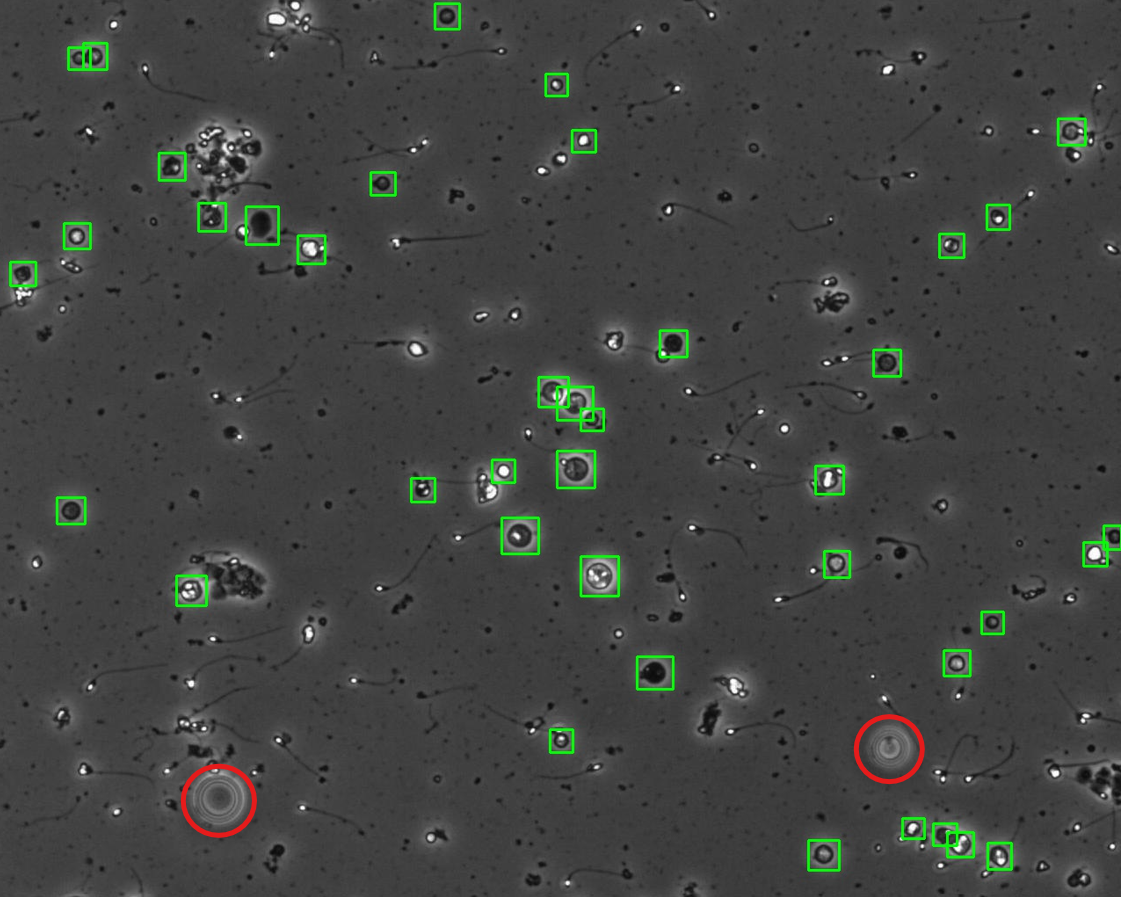
\includegraphics[width=1.0\textwidth]{figuras/rounds_cells/Anillos de Newton.png}
  \caption{Ilustración con Anillos de Newton}
  \label{fig:Anillos_Newton}
\end{figure}

Asimismo, en la imagen \ref{fig:feedback_experto} se evidencian las constantes dudas a cerca de las deteciones decélulas, no solo por el personal que define el proyecto sino por los propios expertos. Cuyo feedback 
"La mayoría de células marcadas con los rectángulos verdes son ciertas células redondas. Los círculos rosas también serían células (probablemente germinales, pero se necesitaría hacer una evaluación morfológica específica para saberlo). 
Los círculos azules, marcan correctamente algunas células redondas pero también indican espermatozoides que retienen la mayor parte del citoplasma (esferas grises con un área blanca bien contrastada). 
En cuanto a los círculos naranjas, muchos son cabezas de espermatozoides sin cola y las eferas más pequeñas desconocemos que son". Esto nos demuestra,
una vez más, el alto grado de complejidad que supone anotar este tipo de imágenes médicas.

\begin{figure}[htbp]
  \centering
  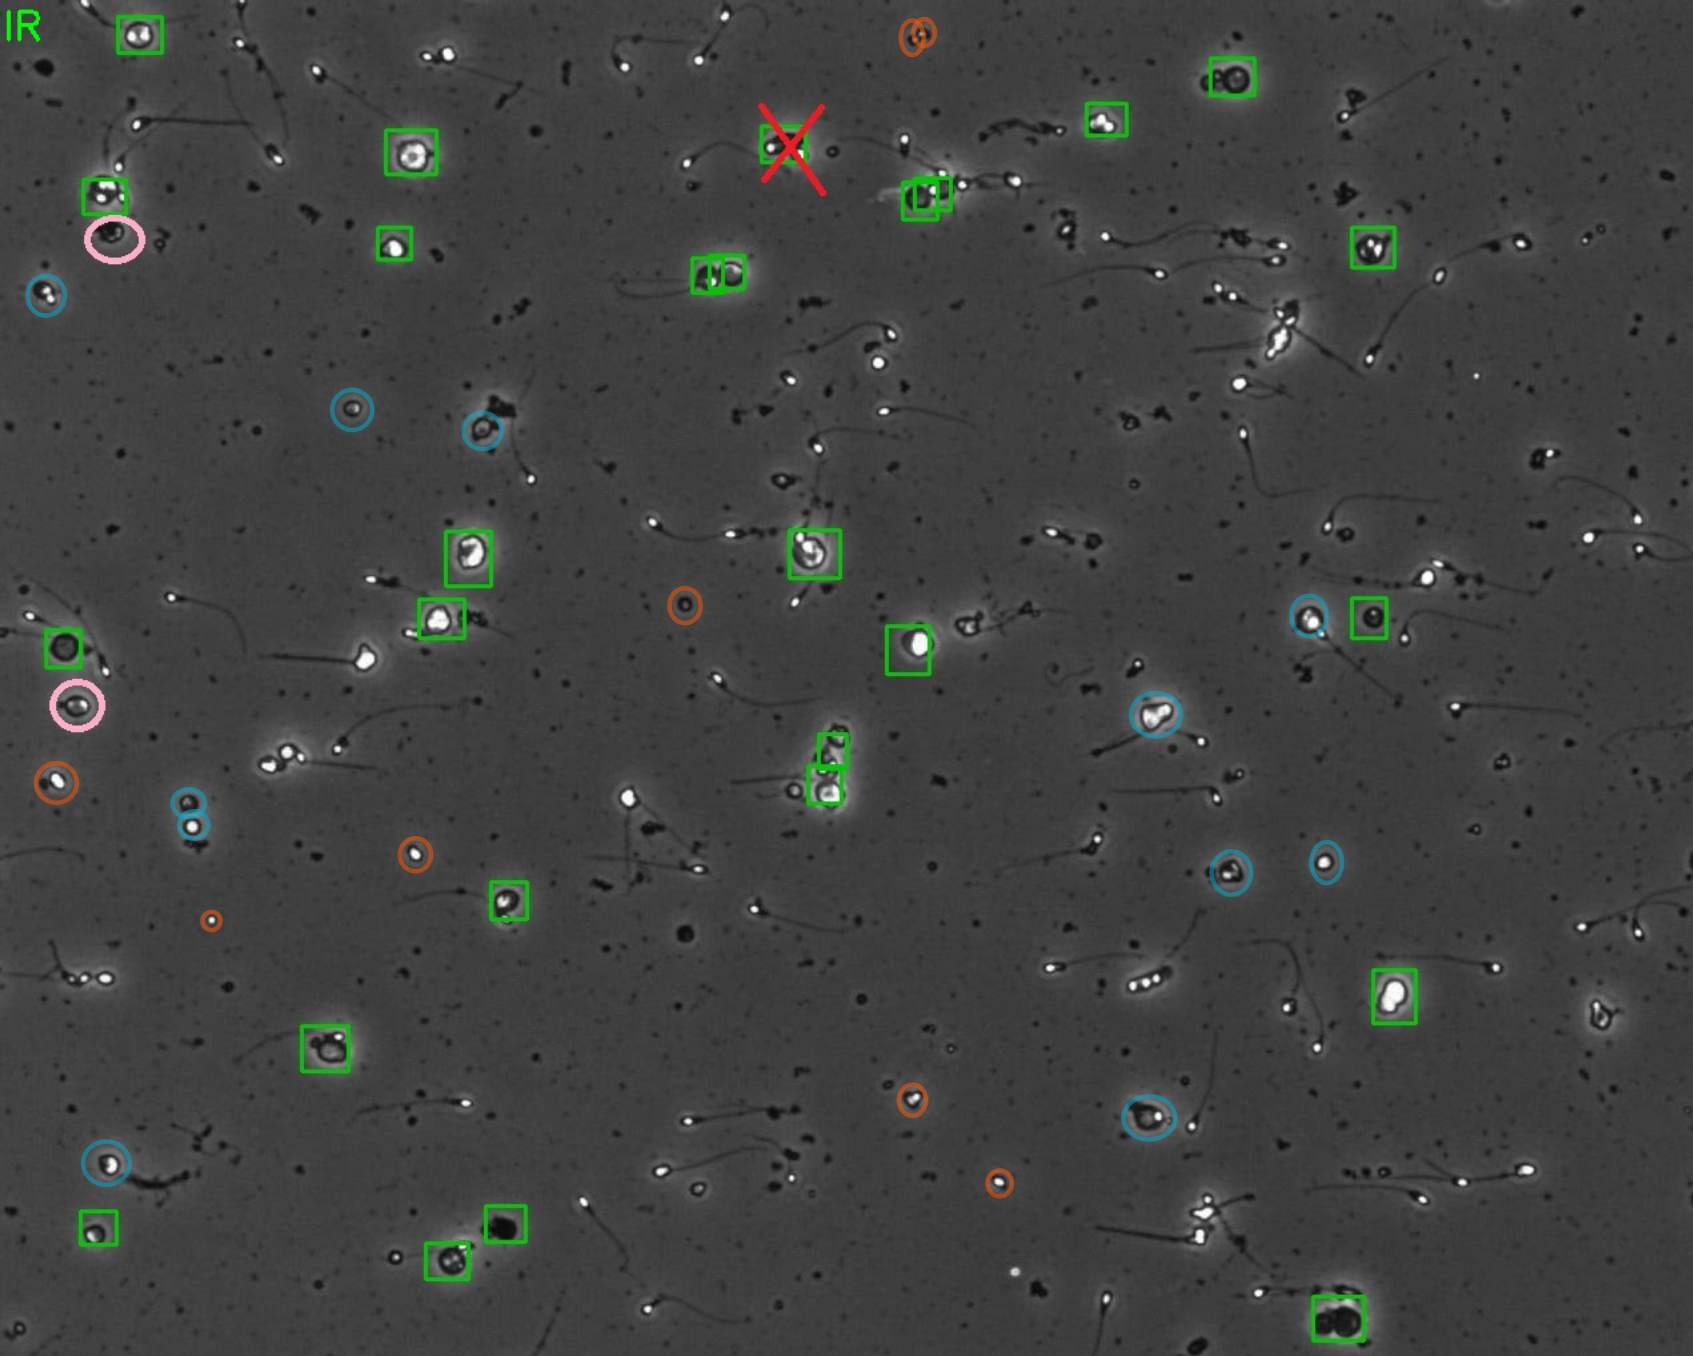
\includegraphics[width=1.0\textwidth]{figuras/rounds_cells/feedback_experto.png}
  \caption{Ilustración de annotaciones para \textit{feedback} con experto}
  \label{fig:feedback_experto}
\end{figure}

\chapter{Gestión de proyecto software} %%%%%%%%%%%%%%%%%%%%%%%%%%%%%%%%%%%%%%%%%%%%%%%%%%%%%%%
\label{Gestión de proyecto software}

\section{Alcance del proyecto}
\label{Alcance del proyecto}

\subsection{Definición del proyecto}

\subsection{Presupuesto}

\subsubsection{Coste de personal}

\subsubsection{Coste del hardware}

\subsubsection{Costes indirectos}

\subsubsection{Coste total}

\section{Plan de trabajo}
\label{Plan de trabajo}

\subsection{Metodología}
\label{Metodología}

\subsection{Identificación de tareas}
\label{Identificación de tareas}

\subsection{Estimación de tareas}
\label{Estimación de tareas}

\subsection{Planificación de tareas}
\label{Planificación de tareas}

\section{Gestión de recursos}
\label{Gestión de recursos}

\subsection{Especificación y asignación de recursos}
\label{Especificación y asignación de recursos}

\section{Gestión de riesgos}
\label{sec:Gestión de riesgos}
\subsection{Identificación y análisis de riesgos}

\clearpage
\section{Legislación y normativa}
\label{Legislación y normativa}

En el marco de ejecución de este proyecto, se ha llevado a cabo un riguroso cumplimiento de la legislación y normativa vigente. A continuación, 
se detalla cómo el proyecto se ajusta y adhiere a las leyes pertinentes:

\begin{itemize}
    \item \textbf{Ley Orgánica 3/2018, de 5 de diciembre, de Protección de Datos Personales y garantía de los derechos digitales}\cite{LOPD2018}
    
    Este proyecto respeta plenamente la Ley Orgánica 3/2018, la cual reconoce el derecho fundamental a la protección de datos personales. 
    La creación y tratamiento del dataset de imágenes médicas se ha realizado conforme a las disposiciones de la ley, asegurando la legalidad en el tratamiento de datos biomédicos. 
    Se han obtenido los permisos explícitos necesarios para el uso de las imágenes, garantizando la privacidad y anonimización de los datos de los pacientes. 
    
    \item \textbf{Reglamento (UE) 2016/679 del Parlamento Europeo y del Consejo relativo a la protección de las personas físicas en lo que respecta al tratamiento de datos personales y a la libre circulación de estos datos (RGPD)}\cite{RGPD2016}

    La creación y tratamiento del dataset de imágenes médicas en este proyecto, se ha realizado conforme a los principios del RGPD, garantizando la legalidad, transparencia en el 
    tratamiento de datos biomédicos. Todas las imágenes han sido previamente anonimizadas y se han implementado medidas técnicas y organizativas 
    para asegurar la seguridad y privacidad de los datos, cumpliendo así con las exigencias del RGPD para datos de salud considerados de categoría 
    especial.
    
    \item \textbf{Reglamento (UE) 2024/1689 del Parlamento Europeo y del Consejo sobre Inteligencia Artificial}\cite{ReglamentoIA2024}

    Este reglamento establece normas armonizadas para garantizar la seguridad, ética y transparencia en el desarrollo y aplicación de sistemas de IA en la Unión Europea.  
    En el contexto de este TFM, el sistema desarrollado se considera una herramienta de investigación y apoyo a la evaluación biomédica —no está concebido ni validado para toma de decisiones clínicas autónomas— 
    por lo que su uso actual no se presenta como IA de alto riesgo. No obstante, para alinearse con los requisitos se incorporan las siguientes medidas: documentación completa, evaluación de riesgos y validación, 
    trazabilidad y registro para una posterior reproducibilidad.
    
    \item \textbf{Real Decreto Legislativo 1/1996 sobre Propiedad Intelectual}\cite{RDL1996}
    
    En conformidad con el Real Decreto Legislativo 1/1996, el proyecto respeta la normativa sobre propiedad intelectual. Se ha optado por utilizar 
    únicamente código y herramientas de software libre y de código abierto para garantizar el cumplimiento de la normativa en materia de propiedad 
    intelectual.

\end{itemize}


\chapter{Metodología} %%%%%%%%%%%%%%%%%%%%%%%%%%%%%%%%%%%%%%%%%%%%%%%%%%%%%%%
\label{metodologia}

En esta sección se describen de forma reproducible los cuatro pipelines experimentales implementados: 
(1) Preprocesado del \textit{dataset}, 
(2) YOLO
(3) Ensamblado (Ensemble). 
(4) Modelo personalizado.

Aquí tengo que hablar de la arquitectura del código.

\section{Preprocesado del \textit{dataset}}
\label{sec:Preprocesado del dataset}
\section{YOLO}
\label{sec:YOLO}
\section{Ensamblado (Ensemble)}
\label{sec:Ensamblado}
\section{Modelo personalizado}
\label{sec:Modelo personalizado}


\chapter{Experimentación} %%%%%%%%%%%%%%%%%%%%%%%%%%%%%%%%%%%%%%%%%%%%%%%%%%%%%%%
\label{Experimentación}

\section{Dataset}
\label{sec:Dataset}
El dataset inicial proporcionado por la empresa MICROPTIC está constituido por un conjunto de \textit{train} y \textit{test} en formato PascalVOC.

\begin{table}[htbp]
\centering
\begingroup
\setlength{\tabcolsep}{8pt}
\small
\begin{adjustbox}{max width=\textwidth}
\begin{tabular}{l c c c c c}
\toprule
Partición & Resoluciones (px) & Nº imágenes (resolución) & Nº imágenes & Sin instancias & Escala grises\\
\midrule
\textit{Train} & \makecell[l]{1280\,×\,1024 \\ 768\,×\,616} & \makecell[r]{356 \\ 17} & 373 & 23 & 3 canales\\ 
\textit{Test}  & \makecell[l]{1280\,×\,1024 \\ 768\,×\,616} & \makecell[r]{87 \\ 7}   & 94  & 6  & 3 canales\\ 
\bottomrule
\end{tabular}
\end{adjustbox}
\endgroup
\caption{Distribución del dataset original}
\label{tab:dataset_original}
\end{table}

El conjunto de datos inicial que nos proporciona Microptic \cite{microptic} está compuesto por 373 imágenes para \textit{train} y 94 para \textit{test}; de las cuales no presentan anotaciones: 23 imágenes de \textit{train} y 6 de \textit{test}.
El conjunto de entrenamiento se divide utilizando la función \texttt{train\_test\_split} de \textit{scikit-learn}, reservando el $80\%$ (298 imágenes) para entrenamiento y el $20\%$ (75 imágenes) para validación. 
Esta división se realiza de forma aleatoria pero reproducible, fijando la semilla (\texttt{random\_state = 42}) para garantizar la consistencia de los resultados.

Adicionalmente, la empresa proporciona un conjunto de datos del \textit{test} reevaluado por expertos del dominio. Este conjunto se reetiqueta utilizando la herramienta \textit{LabelImg} \cite{labelimg_github} en formato PascalVOC. 
Las correcciones afectan a un total de 60 imágenes, incrementando el número de instancias de 1273 a 1412.

Asimismo, se incluyeron dos conjuntos adicionales denominados \textit{test2} y \textit{test3}, inicialmente sin anotaciones pero que contenían \textit{bounding boxes} generados por modelos YOLO preentrenados 
por el grupo GVIS de la Universidad de León. Estas predicciones fueron posteriormente corregidas y validadas por expertos, proporcionando dos conjuntos adicionales para evaluación. 
La composición final del dataset se presenta en la Tabla~\ref{tab:dataset_final}.

\clearpage
\begin{table}[htbp]
\centering
\rowcolors{2}{gray!12}{white}
\begin{tabular}{l c c c c c}
\toprule
Partición & Imágenes & Instancias & 1280$\times$1024 & 768$\times$616 & Escala grises\\
\midrule
\textit{Train}          & 298 & 3934 & 282 & 16 & 3 canales\\
\textit{Validation}     &  75 &  878 & 74  & 1  & 3 canales\\
\textit{Original\_test} &  94 & 1273 & 87  & 7  & 3 canales\\
\textit{Test}           &  94 & 1412 & 87  & 7  & 3 canales\\
\textit{Test2}          &  10 &  144 & 0   & 10 & 1 canal\\
\textit{Test3}          &  59 & 1135 & 56  & 3  & 1 canal\\
\bottomrule
\end{tabular}
\caption{Resumen del dataset de actuación}
\label{tab:dataset_final}
\end{table}

El conjunto de \textit{train}, \textit{validation} y \textit{test} están constituidos por imágenes RGB de 3 canales, mientras que las imágenes 
de los conjuntos de \textit{test2} y \textit{test3} están compuestos por imágenes en escala de grises de un único canal. 

Para el entrenamiento de diferentes arquitecturas de detección de objetos, se convierten los formatos de PascaVOC a YOLO y YOLO a COCO. 
Para más deralle, la información relativa al preprocesamiento del dataset se encuentra en el documento \texttt{preprocesamiento.ipynb} del repositorio \cite{repoTFM}.

\section{Entorno de desarrollo}
\label{sec:Entorno de desarrollo}
Se utilizan dos entornos de desarrrollo complementarios, garantizando la reproducibilidad y escalabilidad de los resultados obtenidos.

\subsection{\textit{Hardware}}
\subsubsection{Hardware Local}
El entorno principal de desarrollo es un equipo \textit{Lenovo IdeaPad Gaming 3} con las siguientes especificaciones técnicas:

\begin{itemize}
    \item \textbf{Procesador}: AMD Ryzen 5 5600H with Radeon Graphics
    \begin{itemize}
        \item Velocidad base: 3,30 GHz
        \item Núcleos físicos: 6
        \item Procesadores lógicos: 12
        \item Caché L1: 384 kB
        \item Caché L2: 3,0 MB  
        \item Caché L3: 16,0 MB
        \item Virtualización: Habilitada
    \end{itemize}
    
    \item \textbf{GPU}: NVIDIA GeForce RTX 3050 Laptop GPU
    \begin{itemize}
        \item Memoria dedicada: 4,0 GB GDDR6
        \item Arquitectura: Ampere
        \item Soporte CUDA: 12.9
        \item Driver version: 576.02
    \end{itemize}
    
    \item \textbf{Memoria RAM}: 16 GB DDR4 SODIMM
    \begin{itemize}
        \item Velocidad: 3200 MHz
        \item Configuración: 2 módulos de 8 GB
    \end{itemize}
    
    \item \textbf{Almacenamiento}: SSD NVMe PCIe Gen3 x4
    \begin{itemize}
        \item Capacidad: 512 GB
        \item Modelo: Micron MTFDHBA512QFD
    \end{itemize}
\end{itemize}

\subsubsection{Servidor privado}
Como entorno complementario se ha empleado un servidor remoto proporcionado por del grupo GVIS de la Universidad de León.

\begin{itemize}
    \item \textbf{GPU}: Tesla T4 con 15 GB de memoria
    \item \textbf{RAM del sistema}: 12,7 GB
    \item \textbf{Almacenamiento temporal}: 78,2 GB SSD
\end{itemize}

\subsection{\textit{Software y Frameworks}}

El desarrollo se realizó empleando el siguiente \textit{stack} tecnológico:

\begin{itemize}
    \item \textbf{Sistema Operativo}: Windows 11
    \item \textbf{Entorno Python}: Miniconda3 (entorno \texttt{TFM})
    \item \textbf{IDE}: Microsoft Visual Studio Code
    \item \textbf{CUDA Toolkit}: Versión 12.9
    \item \textbf{Frameworks principales}:
    \begin{itemize}
        \item PyTorch 2.6.0 con soporte CUDA 12.6
        \item Ultralytics 8.3.177
        \item OpenCV para procesamiento de imágenes
        \item Optuna para optimización de hiperparámetros
        \item Streamlit para desarrollo de interfaces web
        \item Pandas para análisis y manipulación de datos
        \item Matplotlib para visualización de datos 
        \item Scikit-learn para métricas y otras utilidades de \textit{machine learning}
        \item Jupyter Notebook para desarrollo y análisis interactivo
        \item linter ruff para mantener un código limpio, coherente y más fácil de mantener.
    \end{itemize}
\end{itemize}

Para el despliegue del proyecto se recomienda tener todas las dependencias del \texttt{requirements.txt} \cite{repoTFM}, el cual 
recoge todas las librerías y versiones necesarias para la correcta ejecución del entorno.

\section{Configuraciones}
\label{sec:Configuraciones}
\subsection{Entrenamiento}

Aquí tengo que poner una tabla con las configuraciones de entrenamiento para ser recreado y cumplir con las normas éticas.

\begin{table}[H]
\centering
\begin{tabular}{|l|c|c|c|c|c|}
\hline
\textbf{Modelo} & \textbf{Nº Trials} & \textbf{Epoch Optuna} & \textbf{Epoch Train} & \textbf{Batch} & \textbf{Image Size} \\
\hline
yolov8s   & 6  & 25 & 40 & 12 & 704 \\
yolov9s   & 6  & 25 & 40 & 10 & 704 \\
yolov10s  & 6  & 25 & 40 & 10 & 704 \\
yolov11s  & 6  & 25 & 40 & 10 & 704 \\
yolov12s  & 6  & 25 & 40 & 7 & 704 \\
yolov12x  & 5  & 25 & 40 & 7 & 704 \\
custom    & 10 & 25 & 40 & 12 & 704 \\
\hline
\end{tabular}
\caption{Hiperparámetros principales de entrenamiento para cada modelo.}
\end{table}


\begin{table}[H]
\centering
\begin{tabular}{|l|c|c|c|c|c|}
\hline
\textbf{Modelo} & \textbf{lr0} & \textbf{lrf} & \textbf{momentum} & \textbf{weight\_decay} & \textbf{optimizer} \\
\hline
yolov8s   & 0.00540 & 0.00399 & 0.90621 & 0.00010 & SGD \\ \hline
yolov9s   & 0.00023 & 0.00153 & 0.84564 & 0.00033 & AdamW \\
yolov10s  & 0.00540 & 0.00399 & 0.90621 & 0.00010 & SGD \\
yolov11s  & 0.00023 & 0.00153 & 0.84564 & 0.00033 & AdamW \\
yolov12s  & 0.00023 & 0.00932 & 0.91627 & 0.00087 & AdamW \\
custom    & 0.00153 & 0.00111 & 0.89113 & 0.00015 & AdamW \\
\hline
\end{tabular}
\caption{Principales hiperparámetros óptimos seleccionados para cada modelo.}
\end{table}

Hiperparámetros del data augmentation:

\begin{description}
  \item[\textbf{warmup\_epochs}:] 5
  \item[\textbf{warmup\_momentum}:] 0.75
  \item[\textbf{degrees}:] 45
  \item[\textbf{translate}:] 0.1
  \item[\textbf{scale}:] 0.06
  \item[\textbf{flipud}:] 0.5
  \item[\textbf{fliplr}:] 0.5
  \item[\textbf{mosaic}:] 0
  \item[\textbf{close\_mosaic}:] 0
\end{description}


\begin{figure}[htbp]
  \centering
  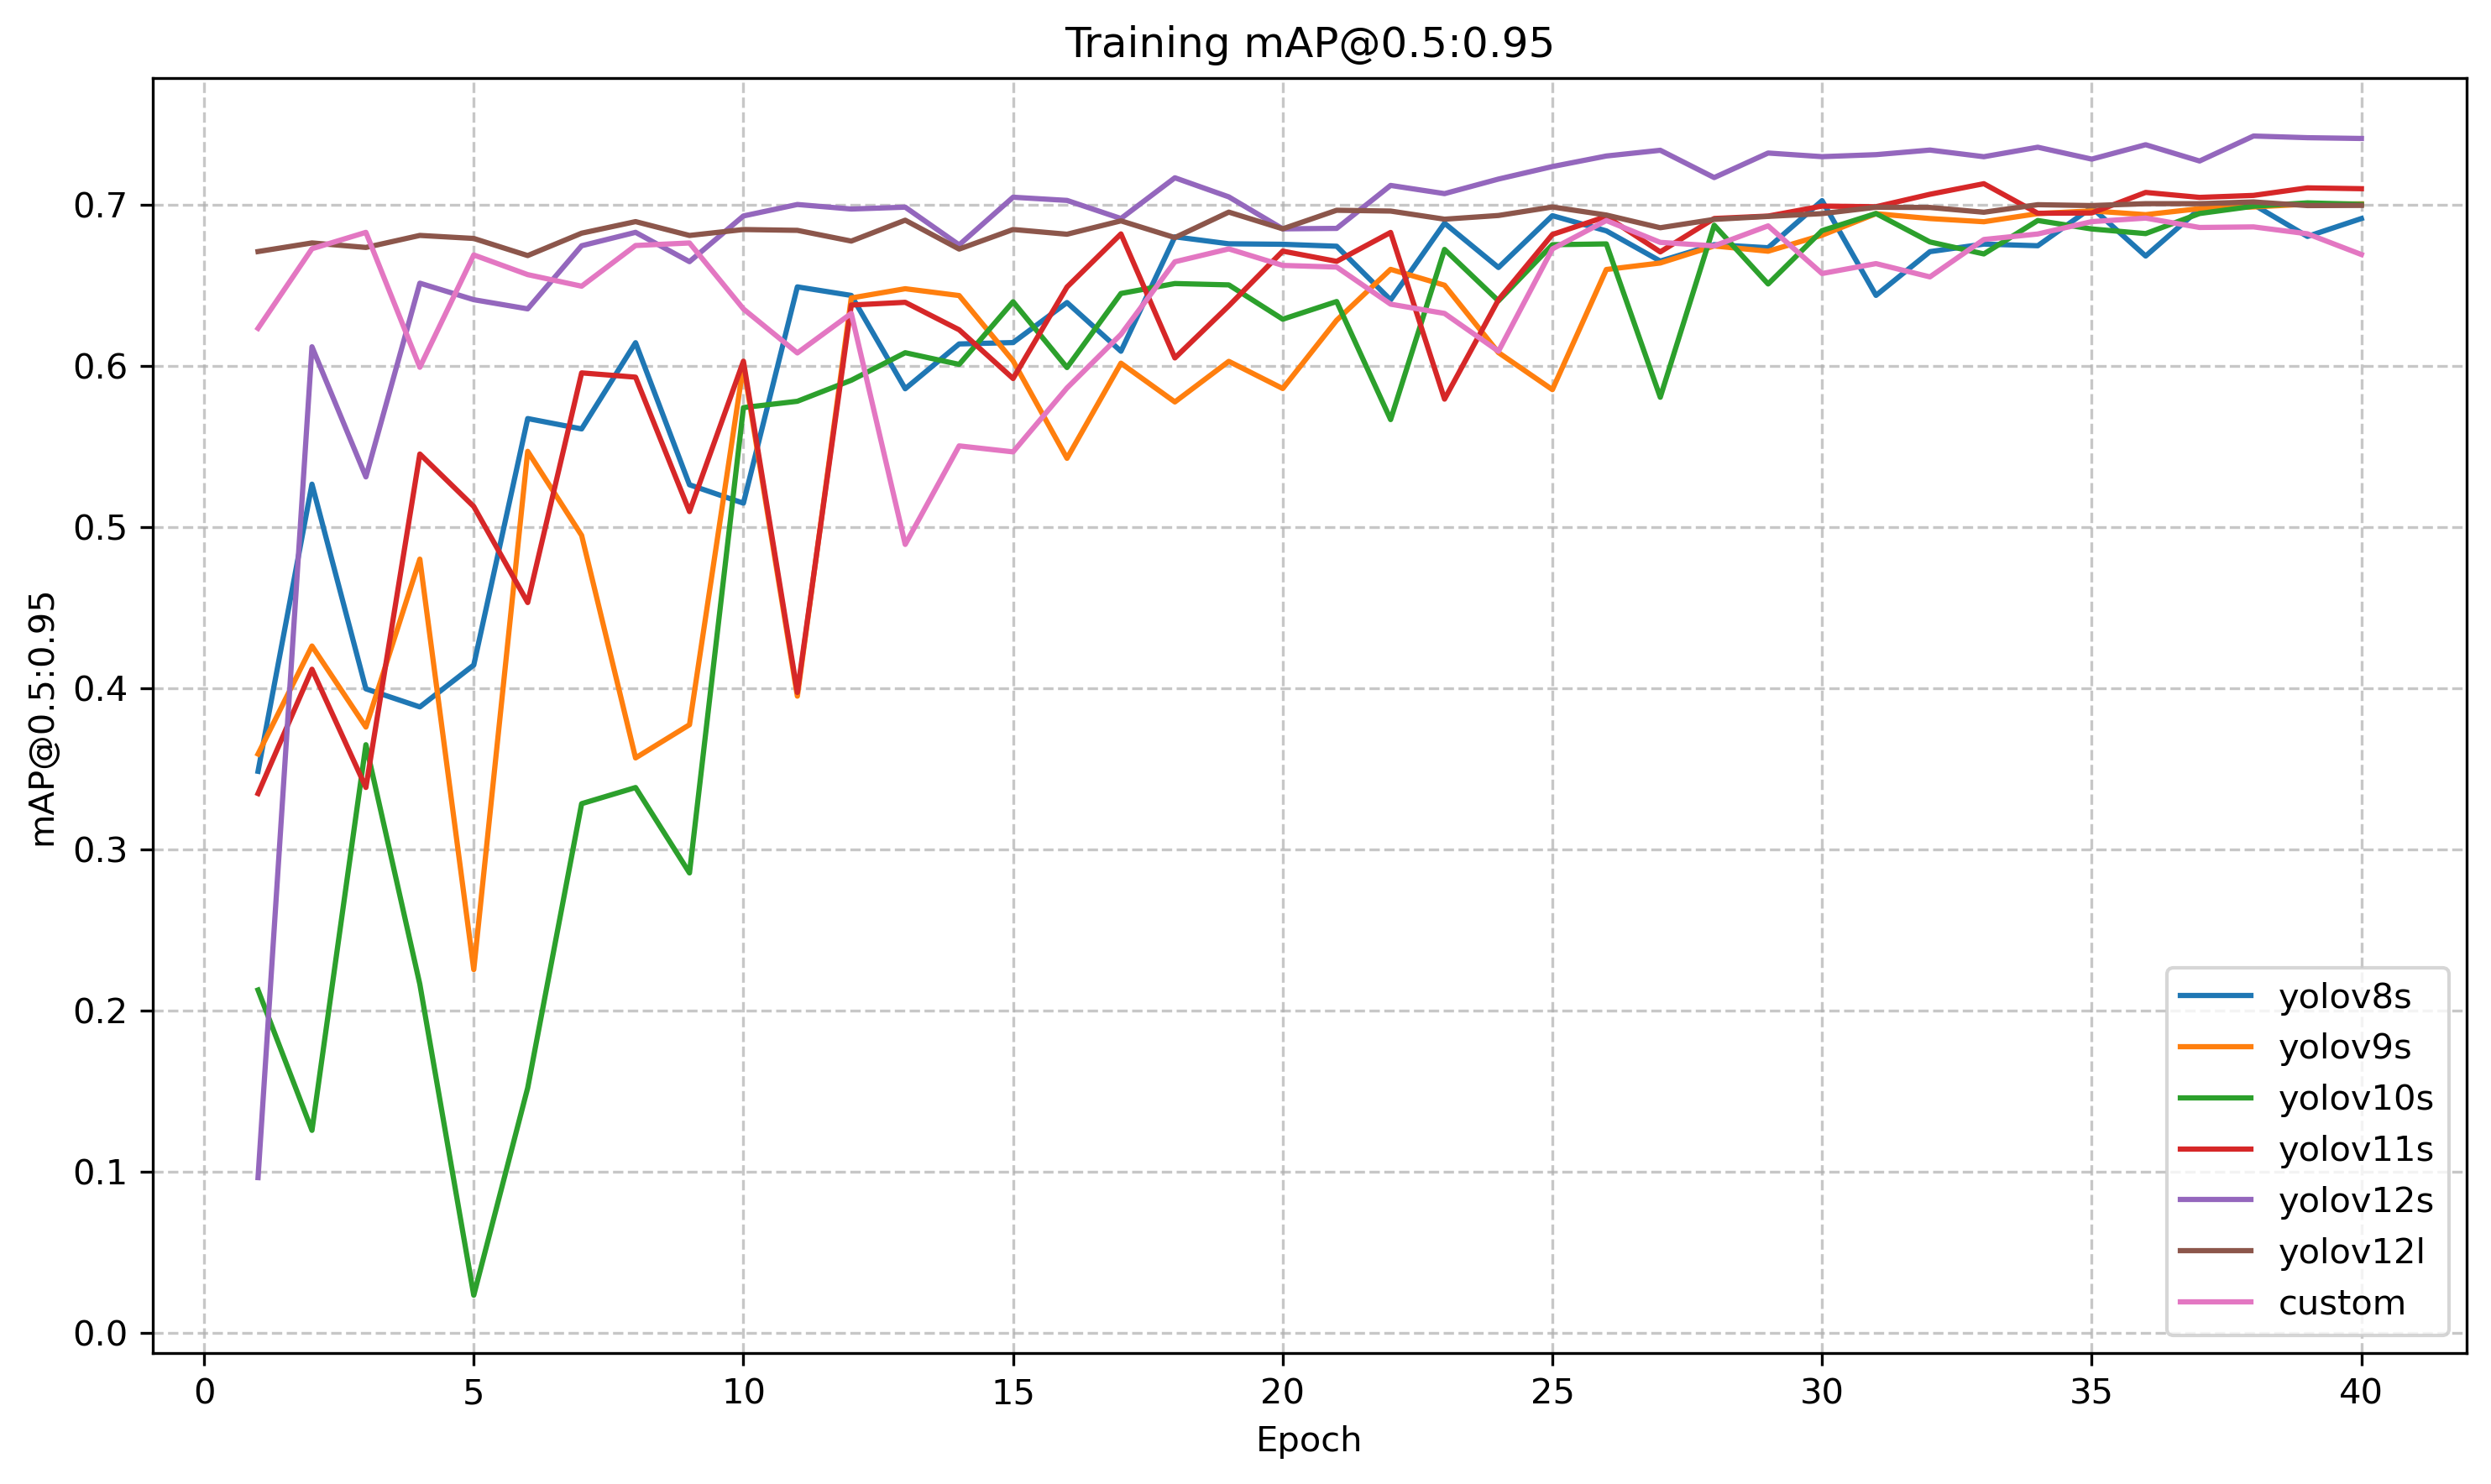
\includegraphics[width=1.0\textwidth]{figuras/yolo_plots/map50-95.png}
  \caption{Interfaz de la aplicación web.}
  \label{fig:yolo_train_map95}
\end{figure}

\begin{figure}[htbp]
  \centering
  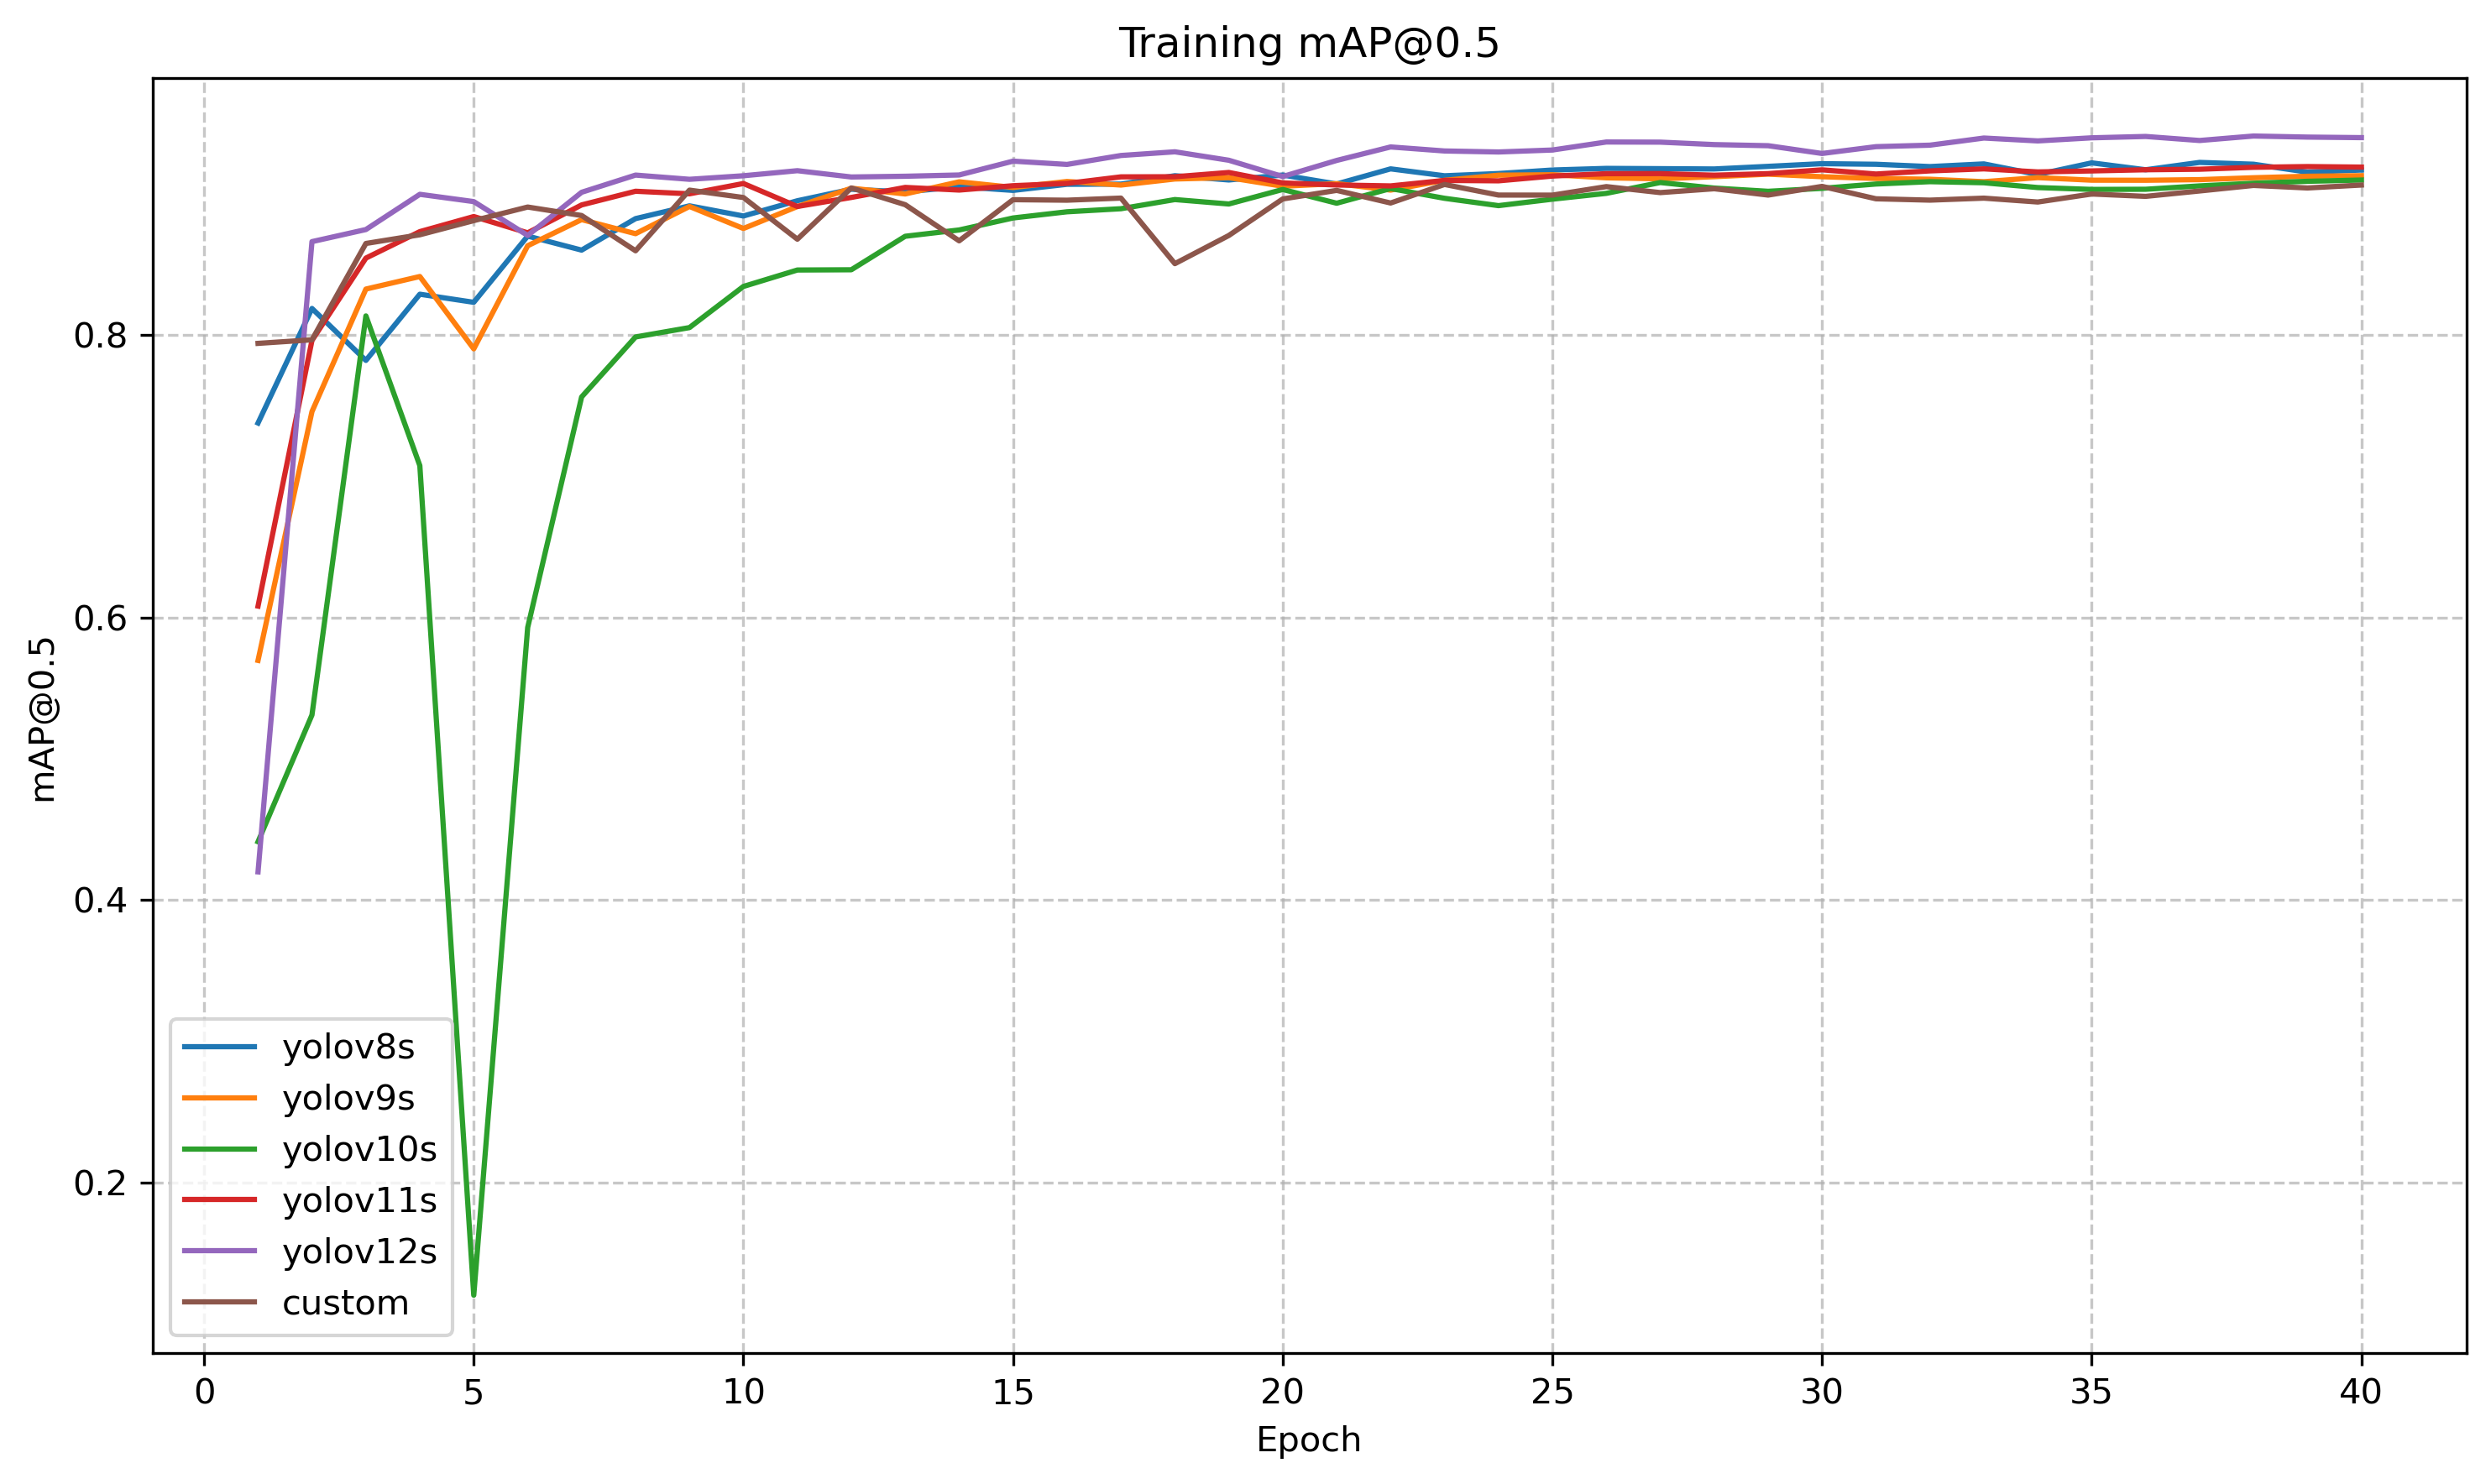
\includegraphics[width=1.0\textwidth]{figuras/yolo_plots/map50.png}
  \caption{Interfaz de la aplicación web.}
  \label{fig:yolo_train_map50}
\end{figure}

\begin{figure}[htbp]
  \centering
  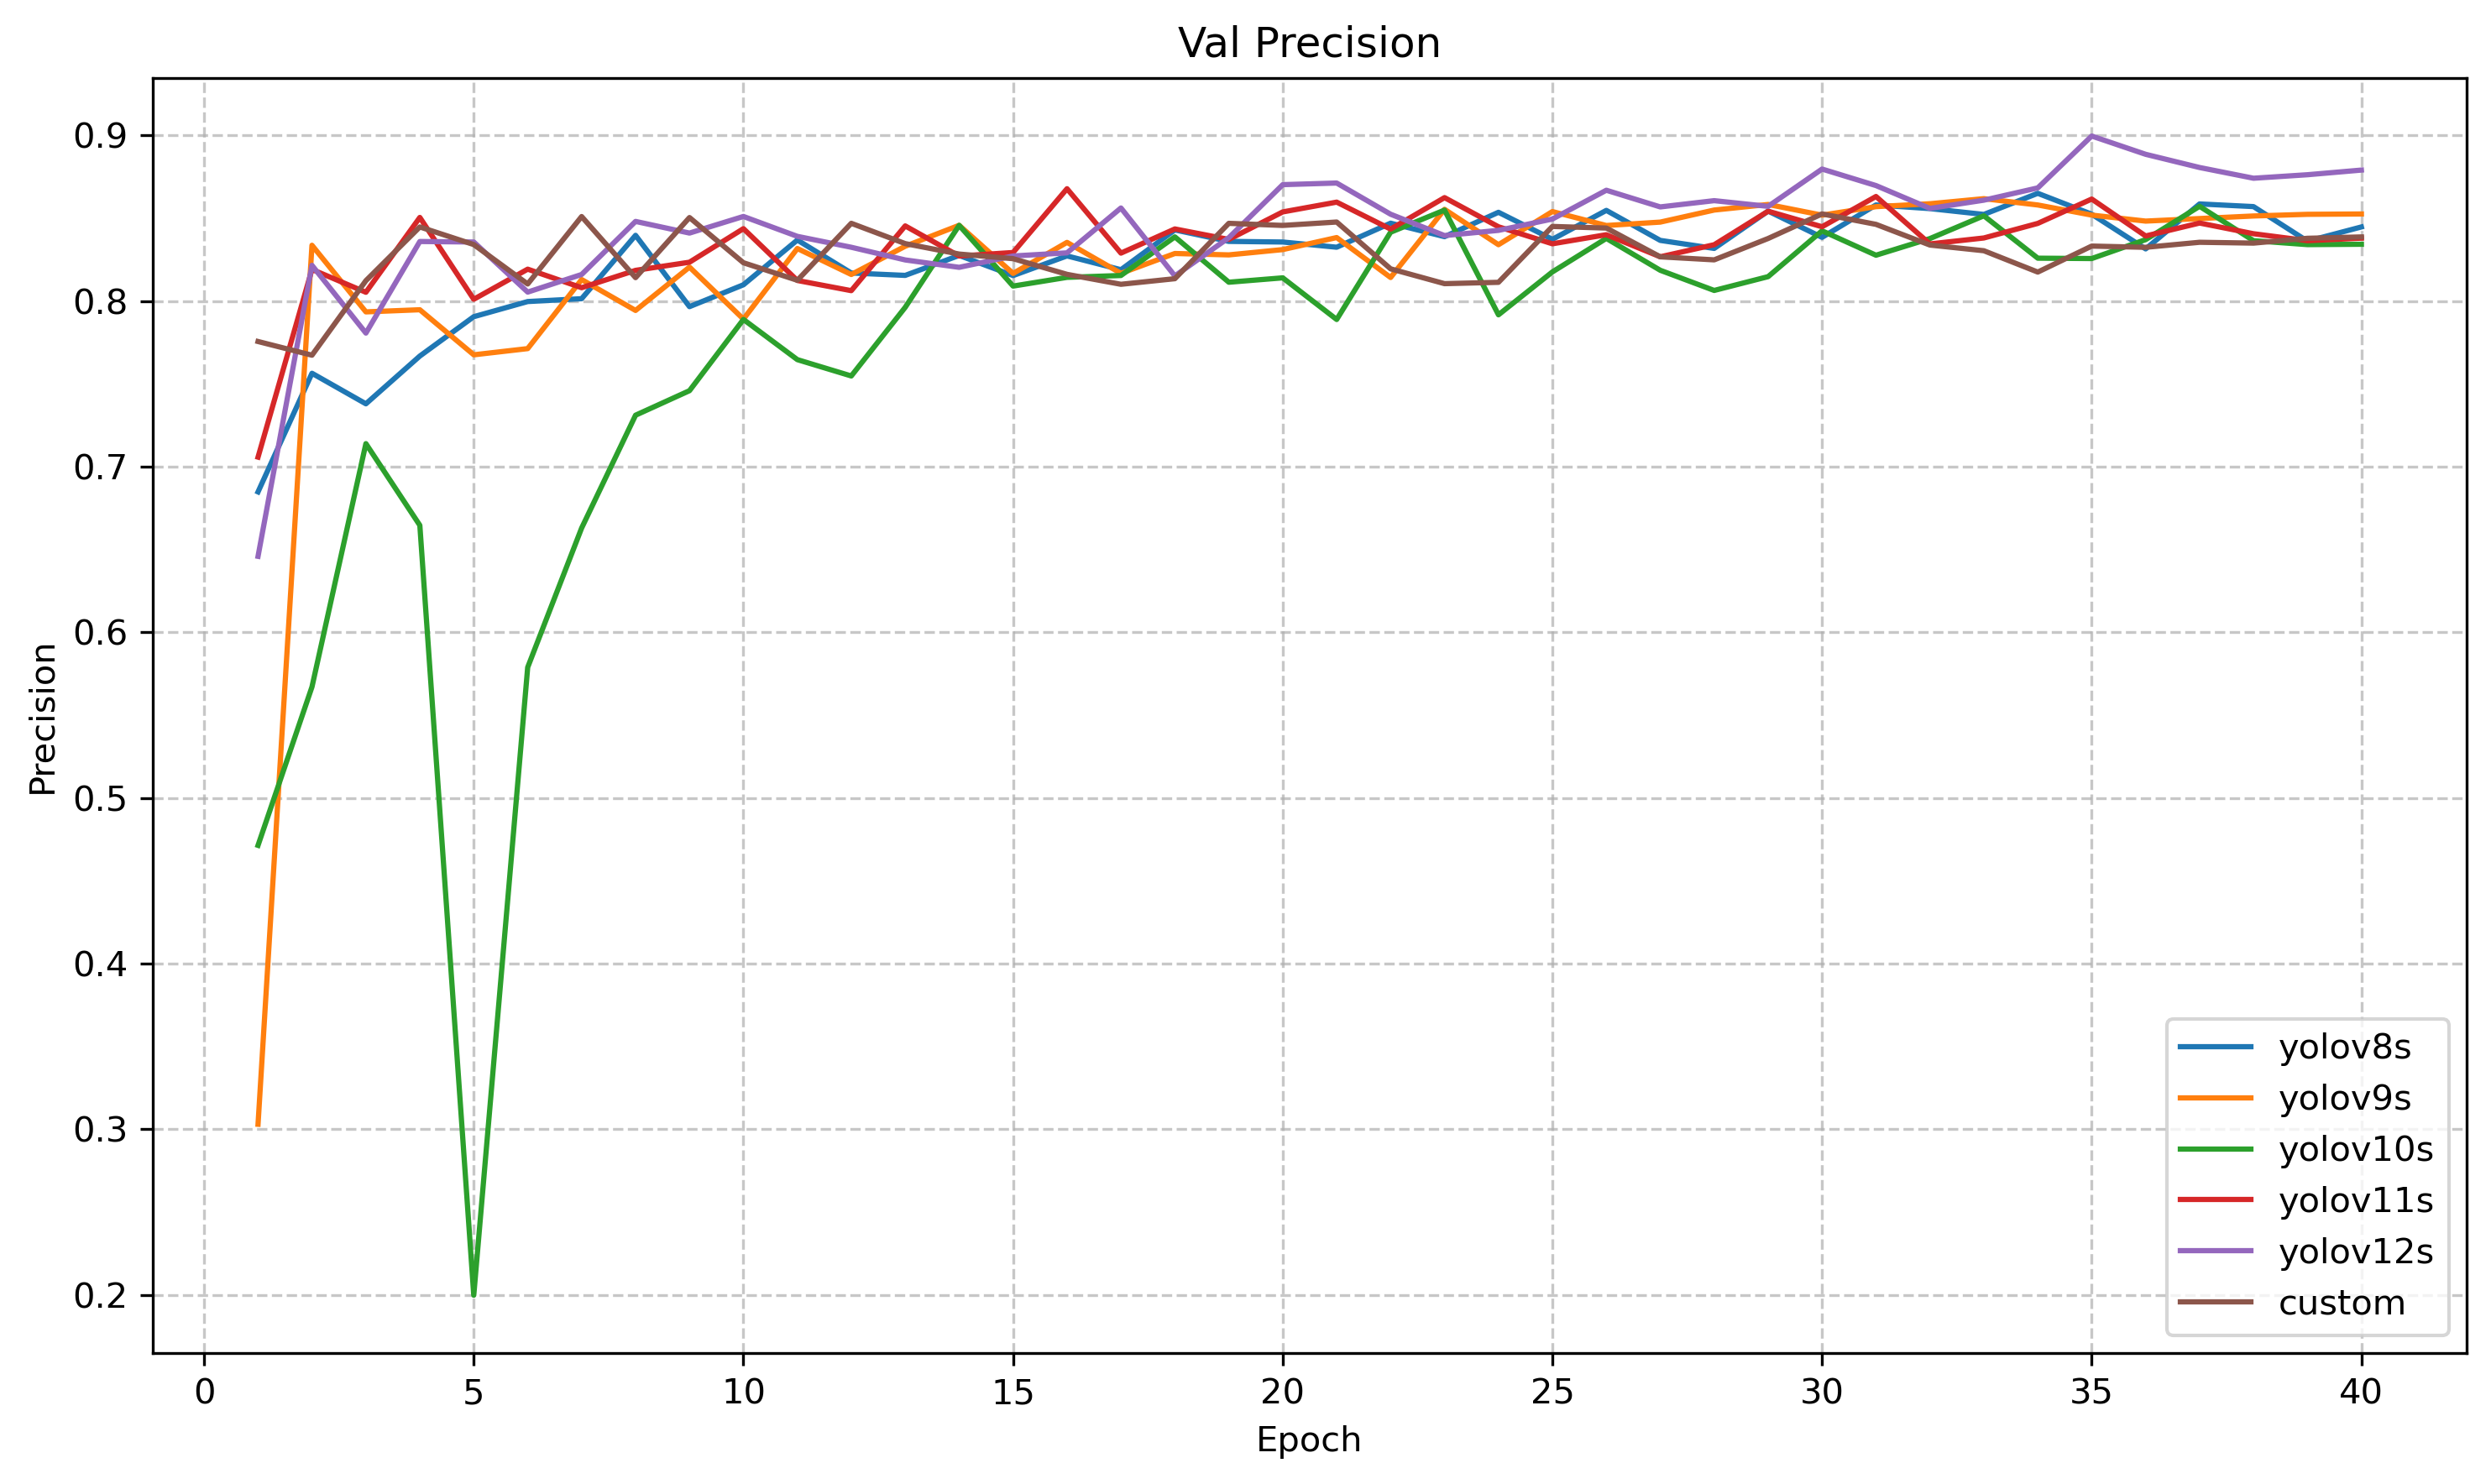
\includegraphics[width=1.0\textwidth]{figuras/yolo_plots/precision.png}
  \caption{Interfaz de la aplicación web.}
  \label{fig:yolo_train_precision}
\end{figure}

\begin{figure}[htbp]
  \centering
  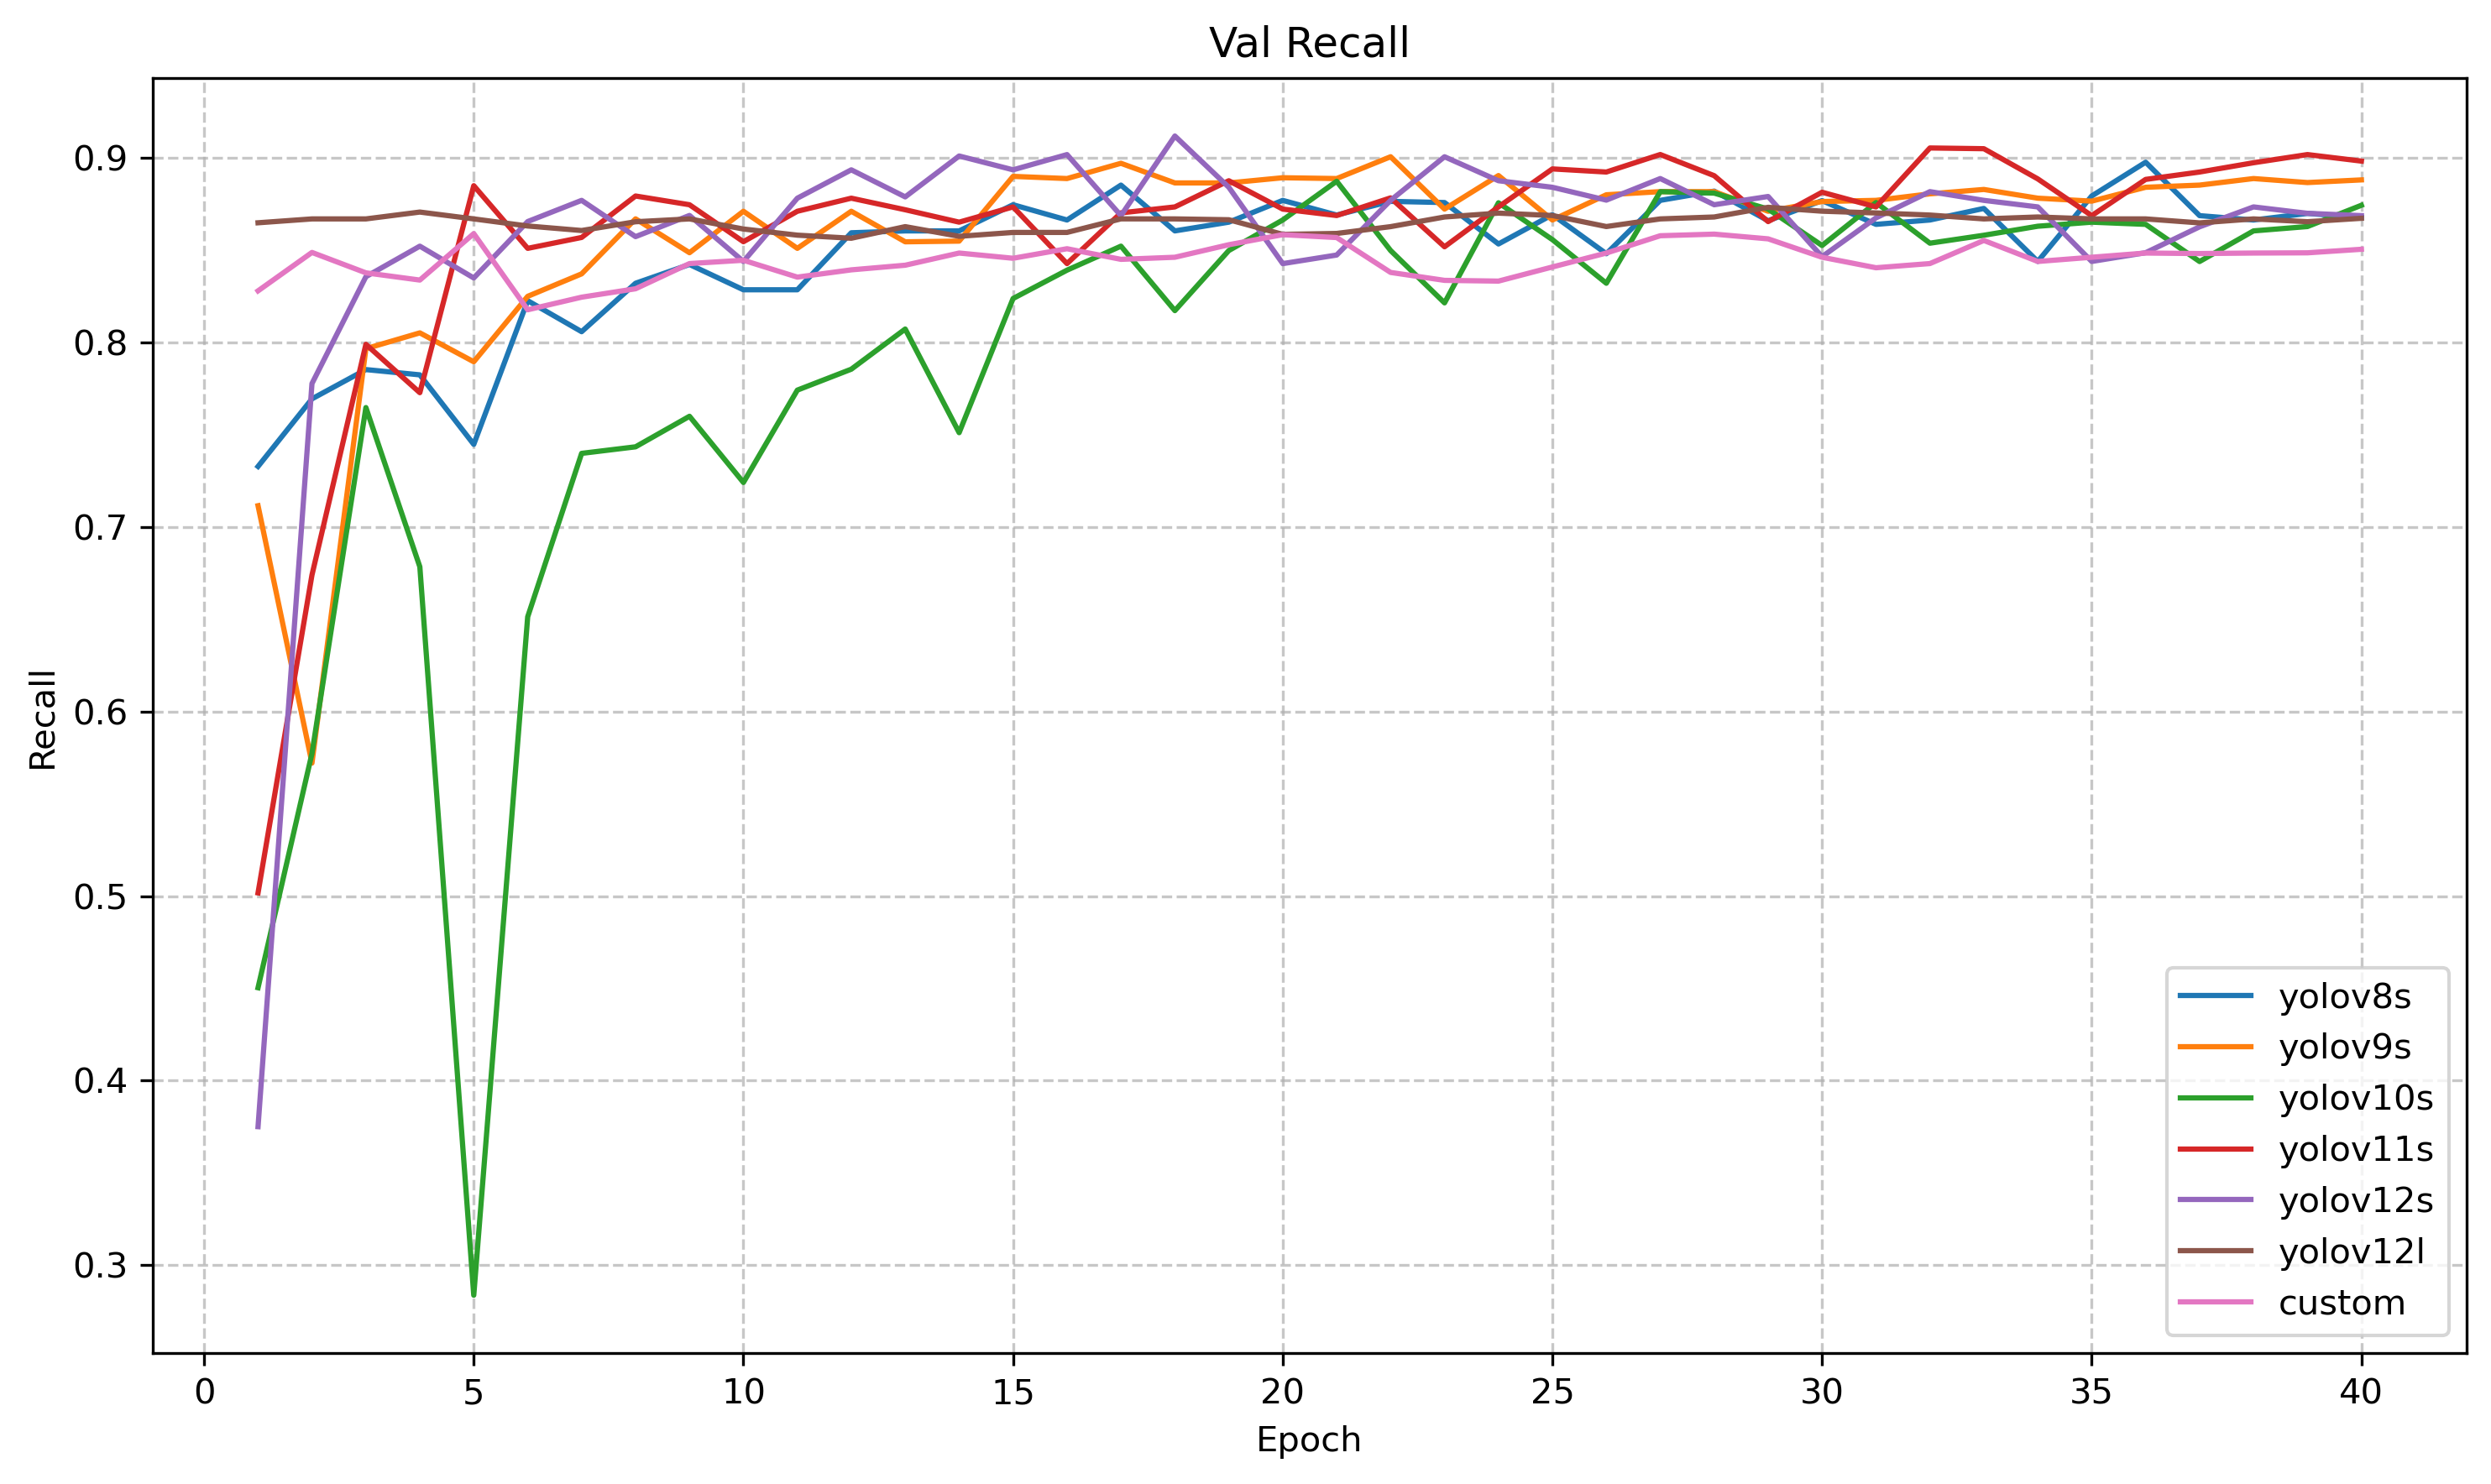
\includegraphics[width=1.0\textwidth]{figuras/yolo_plots/recall.png}
  \caption{Interfaz de la aplicación web.}
  \label{fig:yolo_train_recall}
\end{figure}

\begin{figure}[htbp]
  \centering
  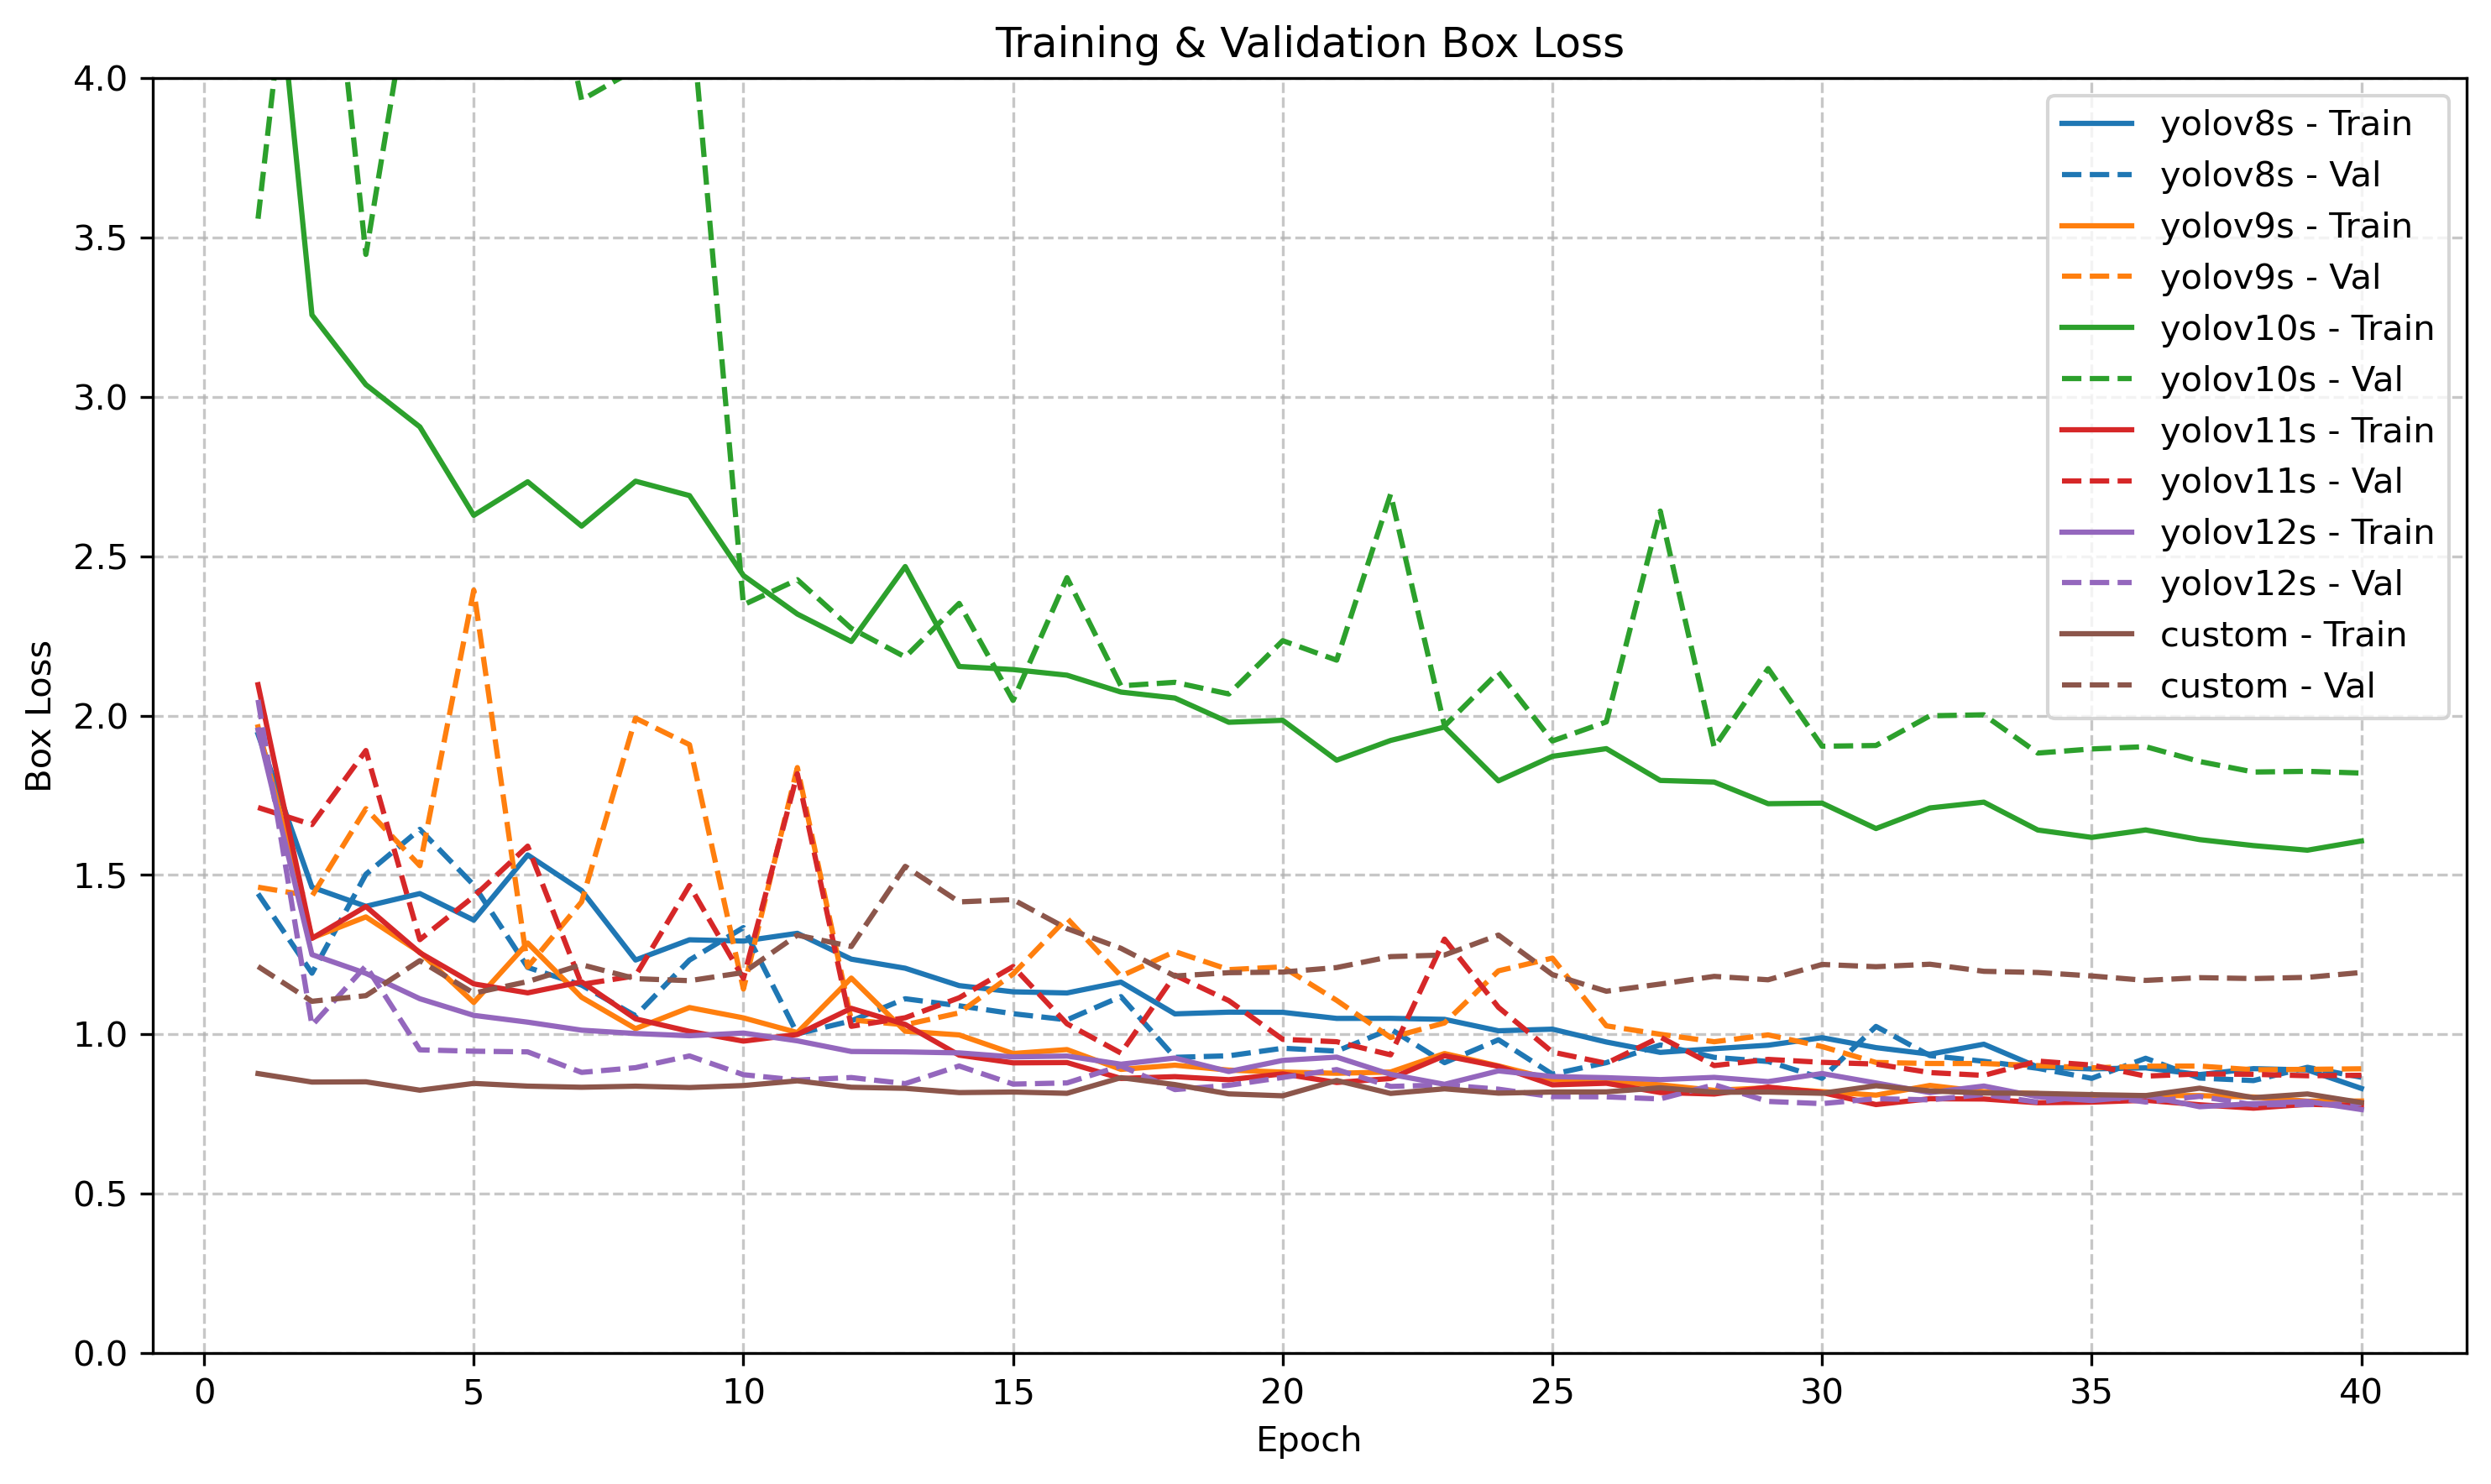
\includegraphics[width=1.0\textwidth]{figuras/yolo_plots/box_loss.png}
  \caption{Interfaz de la aplicación web.}
  \label{fig:yolo_train_box_loss}
\end{figure}

\begin{figure}[htbp]
  \centering
  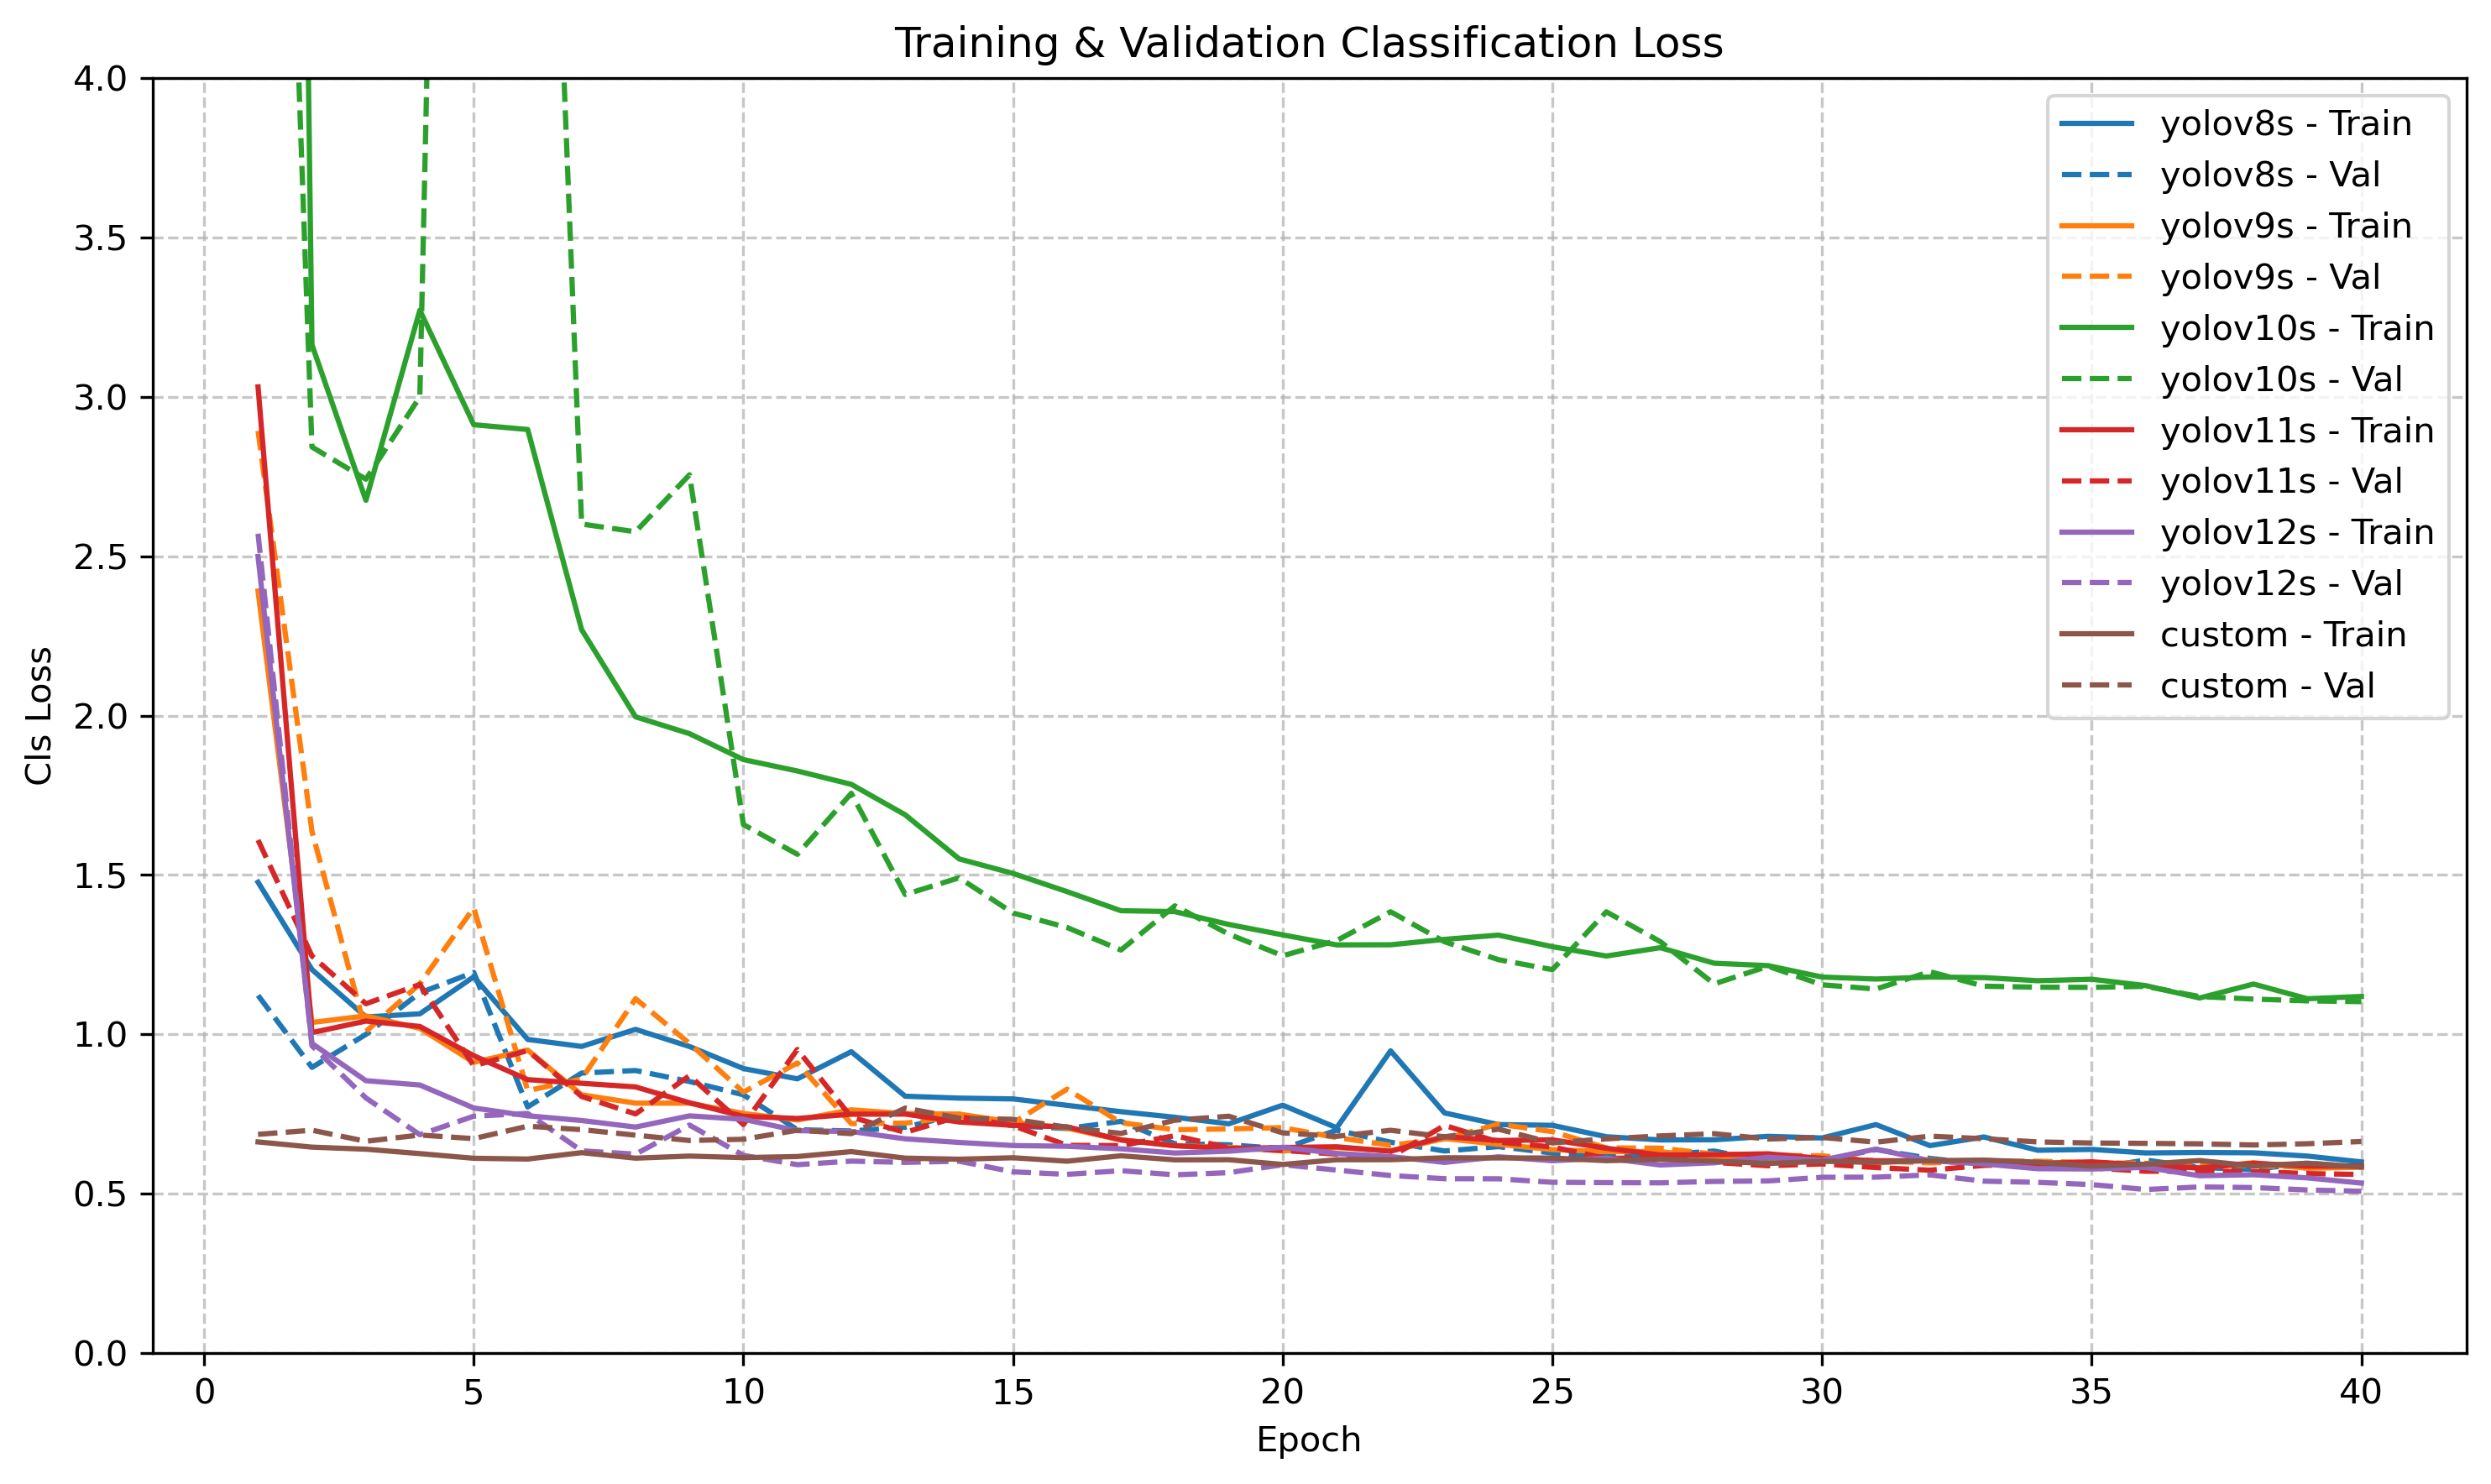
\includegraphics[width=1.0\textwidth]{figuras/yolo_plots/cls_loss.png}
  \caption{Interfaz de la aplicación web.}
  \label{fig:yolo_train_cls_loss}
\end{figure}

\subsection{Validación cruzada}

\section{Métricas}
\label{sec:Métricas}
Para la evaluación de los modelos, se emplea un conjunto de métricas fundamentales que se exponen a continuación.

\begin{description}
  \item[\textit{Precision}] Mide la proporción de detecciones correctas entre todas las detecciones realizadas:
  \[
    \mathrm{Precision} = \frac{TP}{TP + FP}
  \]
  donde TP son los verdaderos positivos y FP los falsos positivos. Alta precision indica pocas detecciones erróneas.

  \item[\textit{Recall}]: Mide la proporción de instancias reales que han sido detectadas:
  \[
    \mathrm{Recall} = \frac{TP}{TP + FN}
  \]
  donde FN son los falsos negativos. Un recall alto indica que el modelo encuentra la mayoría de las instancias reales.

  \item[\textit{mean Average Precision (mAP)}] Para detección de objetos se calcula la curva precision–recall para cada clase y su área bajo la curva (AP). El \textit{mean Average Precision} es la media de las AP sobre todas las clases:
  \[
    \mathrm{mAP} = \frac{1}{C}\sum_{c=1}^{C} \mathrm{AP}_c
  \]
  donde $C$ es el número de clases. En detección se considera una predicción como verdadero positivo si el \textit{Intersection over Union} (IoU) entre la caja predicha y la caja ground truth supera un umbral (por ejemplo IoU $\geq 0.5$). 

  \medskip

  \noindent\textbf{mAP@0.5 (mAP50).} Es la mAP calculada usando un único umbral de IoU igual a 0.5. Formalmente:
  \[
    \mathrm{mAP@0.5} \;=\; \frac{1}{C}\sum_{c=1}^{C} \mathrm{AP}_c(\mathrm{IoU}=0.5)
  \]
  Es una medida menos exigente, que acepta solapamientos moderados entre predicción y \textit{ground truth}.

  \medskip

  \noindent\textbf{mAP@[0.5:0.95] (mAP50:95).} Es la mAP estándar del benchmark COCO que promedia la AP de cada clase sobre múltiples umbrales de IoU desde 0.50 hasta 0.95 con paso 0.05 (10 umbrales: 0.50, 0.55, …, 0.95). Nota: COCO calcula cada AP integrando la curva precision–recall muestreada en 101 puntos, y después se promedian las AP en los 10 umbrales para obtener mAP@[0.5:0.95].
  \[
    \mathrm{mAP}_{[0.5:0.95]} \;=\; \frac{1}{C}\frac{1}{T}\sum_{c=1}^{C}\sum_{t\in\{0.50,0.55,\dots,0.95\}} \mathrm{AP}_c(\mathrm{IoU}=t)
  \]
  donde $T=10$. Esta métrica es más exigente porque penaliza detecciones con IoU bajos y refleja mejor la precisión espacial del modelo.
  \item[Inferencia (ms)] Tiempo medio (en milisegundos) que tarda un modelo en procesar una única imagen (inferencia). Métrica relevante para proyectos en tiempo real.
\end{description}
\arrayrulecolor[HTML]{B9DAE1}


\chapter{Resultados} %%%%%%%%%%%%%%%%%%%%%%%%%%%%%%%%%%%%%%%%%%%%%%%%%%%%%%%
\label{Resultados}

\section{Resultados de los modelos}
\label{sec:Resultados de los modelos}
\subsection{YOLO}

\begin{table}[H]
    \centering
    \resizebox{\textwidth}{!}{
    \begin{tabular}{lccccc}
        \hline
        \textbf{Modelo} & \textbf{Precisión (P)} & \textbf{Recall (R)} & \textbf{mAP@0.5} & \textbf{mAP@0.5:0.95} & \textbf{Inferencia (ms)} \\
        \hline
        YOLOv7      & 0.87  & 0.889 & 0.935 & 0.722 & 20.0   \\
        YOLOv7-W6   & 0.847 & 0.883 & 0.925 & 0.694 & 16.0   \\
        YOLOv7-E6E  & 0.906 & 0.857 & 0.934 & 0.721 & 127.5  \\
        \hline
    \end{tabular}
    }
    \caption{Resultados de los modelos YOLOv7 sobre el conjunto de test original.}
    \label{tab:yolov7_results}
\end{table}

\begin{table}[H]
    \centering
    \resizebox{\textwidth}{!}{
    \begin{tabular}{lccccc}
        \hline
        \textbf{Modelo} & \textbf{Precisión (P)} & \textbf{Recall (R)} & \textbf{mAP@0.5} & \textbf{mAP@0.5:0.95} & \textbf{Inferencia (ms)} \\
        \hline
        yolov8s    & 0.843 & 0.844 & 0.920 & 0.722 & 11.006 \\
        yolov9s    & 0.838 & 0.852 & 0.921 & 0.721 & 13.485 \\
        yolov10s   & 0.821 & 0.867 & 0.918 & 0.717 & 11.221 \\
        yolov11s   & 0.861 & 0.824 & 0.921 & 0.732 & 11.248 \\
        yolov12s   & 0.856 & 0.863 & 0.936 & 0.761 & 14.615 \\
        \hline
    \end{tabular}
    }
    \caption{Resultados de los modelos YOLO sobre el conjunto de test original.}
    \label{tab:yolov8_12_results}
\end{table}

% Tabla para los resultados sobre los conjuntos de Test
\definecolor{turquoise}{RGB}{64,224,208}
\begin{table}[ht]
\centering
\rowcolors{2}{gray!15}{white}
\renewcommand{\arraystretch}{1.3}
\setlength{\arrayrulewidth}{1.2pt}
\resizebox{\textwidth}{!}{
\arrayrulecolor{gray}
\begin{tabular}{!{\vrule width 1.2pt}l|c|c|c|c|c|c!{\vrule width 1.2pt}}
\arrayrulecolor{black}
\specialrule{1.5pt}{0pt}{0pt}
\rowcolor{gray!30}
\textbf{Modelo} & \textbf{Test} & \textbf{Precisión} & \textbf{Recall} & \textbf{mAP@0.5} & \textbf{mAP@0.5:0.95} & \textbf{Inferencia (ms)} \\
\specialrule{1.2pt}{0pt}{0pt}
\arrayrulecolor{gray}
yolov8s   & test & 0.855 & 0.838 & 0.926 & 0.704 & 11.067 \\ \hline
yolov9s   & test & 0.851 & \cellcolor{turquoise!30}0.876 & 0.933 & 0.706 & 12.904 \\ \hline
yolov10s  & test & 0.853 & 0.861 & 0.927 & 0.701 & 11.041 \\ \hline
yolov11s  & test & 0.846 & 0.866 & 0.930 & 0.716 & \cellcolor{turquoise!30}10.644 \\ \hline
yolov12s  & test & \cellcolor{turquoise!30}0.861 & 0.848 & \cellcolor{turquoise!30}0.936 & \cellcolor{turquoise!30}0.740 & 15.066 \\
\arrayrulecolor{black}
\specialrule{1.2pt}{0pt}{0pt}
\arrayrulecolor{gray}
yolov8s & test2 & 0.924 & \cellcolor{turquoise!30}0.938 & 0.969 & 0.553 & 37.858 \\ \hline
yolov9s & test2 & 0.917 & 0.927 & 0.961 & 0.542 & 35.944 \\ \hline
yolov10s & test2 & 0.956 & 0.898 & 0.962 & \cellcolor{turquoise!30}0.589 & \cellcolor{turquoise!30}12.358 \\ \hline
yolov11s & test2 & 0.929 & 0.917 & 0.964 & 0.534 & 14.967 \\ \hline
yolov12s & test2 & \cellcolor{turquoise!30}0.965 & 0.917 & \cellcolor{turquoise!30}0.975 & 0.556 & 20.254 \\
\arrayrulecolor{black}
\specialrule{1.2pt}{0pt}{0pt}
\arrayrulecolor{gray}
yolov8s & test3 & 0.842 & 0.862 & \cellcolor{turquoise!30}0.937 & 0.700 & 11.314 \\ \hline
yolov9s & test3 & 0.843 & 0.870 & 0.935 & 0.681 & 13.291 \\ \hline
yolov10s & test3 & \cellcolor{turquoise!30}0.873 & 0.826 & 0.926 & 0.667 & \cellcolor{turquoise!30}11.109 \\ \hline
yolov11s & test3 & 0.855 & \cellcolor{turquoise!30}0.874 & 0.935 & 0.698 & 12.561 \\ \hline
yolov12s & test3 & 0.836 & 0.821 & 0.922 & \cellcolor{turquoise!30}0.723 & 15.442 \\
\arrayrulecolor{black}
\specialrule{1.5pt}{0pt}{0pt}
\end{tabular}
}
\caption{Evaluación de modelos YOLO sobre los diferentes conjuntos de prueba}
\end{table}

Es importante que hablemos de esta problemática y como evitamos un reetiquetado de imágenes que pueden dar más confusión al confundir clases, y continuar la tendencia monoclase.

% Tabla para los artefactos
\definecolor{mygreen}{RGB}{0,180,0}
\definecolor{myred}{RGB}{220,0,0}
\begin{table}[ht]
\centering 
\resizebox{\textwidth}{!}{%
\begin{tabular}{|c|c|c|c|c|c|c|c|c|c|c|c|}
\hline
\textbf{Imagen} & \textbf{Test} & \textbf{yolov8s 0.5} & \textbf{yolov8s 0.7} & \textbf{yolov9s 0.5} & \textbf{yolov9s 0.7} & \textbf{yolov10s 0.5} & \textbf{yolov10s 0.7} & \textbf{yolov11s 0.5} & \textbf{yolov11s 0.7} & \textbf{yolov12s 0.5} & \textbf{yolov12s 0.7} \\
\hline
59 imagen         & 1 & \cellcolor{myred!30}\ding{55} & \cellcolor{mygreen!30}\ding{51} & \cellcolor{myred!30}\ding{55} & \cellcolor{mygreen!30}\ding{51} & \cellcolor{myred!30}\ding{55} & \cellcolor{mygreen!30}\ding{51} & \cellcolor{mygreen!30}\ding{51} & \cellcolor{mygreen!30}\ding{51} & \cellcolor{mygreen!30}\ding{51} & \cellcolor{mygreen!30}\ding{51} \\
\hline
61 imagen         & 1 & \cellcolor{myred!30}\ding{55} & \cellcolor{mygreen!30}\ding{51} & \cellcolor{myred!30}\ding{55} & \cellcolor{myred!30}\ding{55} & \cellcolor{mygreen!30}\ding{51} & \cellcolor{mygreen!30}\ding{51} & \cellcolor{myred!30}\ding{55} & \cellcolor{mygreen!30}\ding{51} & \cellcolor{mygreen!30}\ding{51} & \cellcolor{mygreen!30}\ding{51} \\
\hline
219 imagen        & 1 & \cellcolor{myred!30}\ding{55} & \cellcolor{mygreen!30}\ding{51} & \cellcolor{myred!30}\ding{55} & \cellcolor{myred!30}\ding{55} & \cellcolor{mygreen!30}\ding{51} & \cellcolor{mygreen!30}\ding{51} & \cellcolor{myred!30}\ding{55} & \cellcolor{mygreen!30}\ding{51} & \cellcolor{mygreen!30}\ding{51} & \cellcolor{mygreen!30}\ding{51} \\
\hline
369 imagen        & 1 & \cellcolor{mygreen!30}\ding{51} & \cellcolor{mygreen!30}\ding{51} & \cellcolor{myred!30}\ding{55} & \cellcolor{myred!30}\ding{55} & \cellcolor{mygreen!30}\ding{51} & \cellcolor{mygreen!30}\ding{51} & \cellcolor{myred!30}\ding{55} & \cellcolor{mygreen!30}\ding{51} & \cellcolor{mygreen!30}\ding{51} & \cellcolor{mygreen!30}\ding{51} \\
\hline
already tested-00 & 3 & \cellcolor{mygreen!30}\ding{51} & \cellcolor{mygreen!30}\ding{51} & \cellcolor{mygreen!30}\ding{51} & \cellcolor{mygreen!30}\ding{51} & \cellcolor{mygreen!30}\ding{51} & \cellcolor{mygreen!30}\ding{51} & \cellcolor{mygreen!30}\ding{51} & \cellcolor{mygreen!30}\ding{51} & \cellcolor{mygreen!30}\ding{51} & \cellcolor{mygreen!30}\ding{51} \\
\hline
already tested-15 & 3 & \cellcolor{mygreen!30}\ding{51} & \cellcolor{mygreen!30}\ding{51} & \cellcolor{myred!30}\ding{55} & \cellcolor{myred!30}\ding{55} & \cellcolor{mygreen!30}\ding{51} & \cellcolor{mygreen!30}\ding{51} & \cellcolor{myred!30}\ding{55} & \cellcolor{mygreen!30}\ding{51} & \cellcolor{mygreen!30}\ding{51} & \cellcolor{mygreen!30}\ding{51} \\
\hline
already tested-16 & 3 & \cellcolor{mygreen!30}\ding{51} & \cellcolor{mygreen!30}\ding{51} & \cellcolor{myred!30}\ding{55} & \cellcolor{mygreen!30}\ding{51} & \cellcolor{mygreen!30}\ding{51} & \cellcolor{mygreen!30}\ding{51} & \cellcolor{mygreen!30}\ding{51} & \cellcolor{mygreen!30}\ding{51} & \cellcolor{mygreen!30}\ding{51} & \cellcolor{mygreen!30}\ding{51} \\
\hline
already tested-17 & 3 & \cellcolor{mygreen!30}\ding{51} & \cellcolor{mygreen!30}\ding{51} & \cellcolor{mygreen!30}\ding{51} & \cellcolor{mygreen!30}\ding{51} & \cellcolor{mygreen!30}\ding{51} & \cellcolor{mygreen!30}\ding{51} & \cellcolor{mygreen!30}\ding{51} & \cellcolor{mygreen!30}\ding{51} & \cellcolor{mygreen!30}\ding{51} & \cellcolor{mygreen!30}\ding{51} \\
\hline
already tested-22 & 3 & \cellcolor{mygreen!30}\ding{51} & \cellcolor{mygreen!30}\ding{51} & \cellcolor{mygreen!30}\ding{51} & \cellcolor{mygreen!30}\ding{51} & \cellcolor{myred!30}\ding{55} & \cellcolor{mygreen!30}\ding{51} & \cellcolor{mygreen!30}\ding{51} & \cellcolor{mygreen!30}\ding{51} & \cellcolor{mygreen!30}\ding{51} & \cellcolor{mygreen!30}\ding{51} \\
\hline
\end{tabular}
}
\caption{Evaluación de modelos YOLO sobre imágenes con artefactos}
\end{table}

\newpage
\subsection{Ensemble}
\subsection{Modelo personalizado}
\section{Discursión de resultados}
\label{sec:Discursión de resultados}


\chapter{Herramienta Web} %%%%%%%%%%%%%%%%%%%%%%%%%%%%%%%%%%%%%%%%%%%%%%%%%%%%%%%
Con el propósito de definir una herramienta de análisis automatizado, se desarrolla una interfaz intuitiva e interactiva para la detección 
de células redondas sobre una muetra individual o colectiva. La información relativa a la aplicación,
se puede encontrar en el manual de usuario (\ref{Manual de usuario}).
\section{Objetivos de la herramienta}
\label{sec:Objetivos de la herramienta}

La herramienta web para la detección de células redondas tiene como principales objetivos:

\begin{itemize}
  \item{\textbf{Detección atomática de células en imágenes microscópicas en el contexto médico abordado con anterioridad:} Permitir identificar
  y localizar células redondas dotando al usuario de diferentes arquitecturas de modelos.}
  \item{\textbf{Comparación de rendimiento entre modelos:} Facilitar la evaluación comparativa entre diferentes modelos
  , permitiendo al usuario seleccionar el mejor modelo y el intervalo de actuación para el IoU.}
  \item{\textbf{Visualización de resultados:} Proporcionar una interface de visualización clara e intuitiva que permita al usuario 
  visualizar las predicciones del modelo y las \textit{bounding boxes} si se dispone de las mismas.}
  \item{\textbf{Análisis cuantitativo:} Permitir obtener métricas y estadísticas como: \textit{precision, accuracy}, conteo o IoU promedio}
  \item{\textbf{Soporte a la investigación biomédica:} Facilitar la identificación temprana de diferentes grados de patología.} 
\end{itemize}

\section{Arquitectura}
\label{sec:Arquitectura}
La arquitectura de la aplicación sigue un diseño modular y escalable basada en \textit{Streamlit}. Esto permite tener una aplicación monolítica que encapsula toda la funcionalidad en un único ejecutable y mantiene 
una clara separación entre la lógica de procesamiento y de presentación.

\subsection{Organización del proyecto}
La estructura principal es:
\begin{itemize}
  \item \texttt{app.py}: orquestación de la interfaz (widgets Streamlit), gestión de sesión y del flujo de inferencia.
  \item \texttt{utils/utils.py}: servicios de \textit{backend} lógico (carga de modelos, preprocesado, inferencia, postprocesado, visualización).
  \item \texttt{assets/styles.css}: estilo e integración visual mediante \texttt{st.markdown}.
  \item \texttt{models/\{final\_model\_yolovXs\}/}: modelos entrenados para la casuística.
  \item \texttt{runs/detect/}: salidas temporales de inferencia (imágenes anotadas, JSON/CSV).
\end{itemize}

Para más información, revisar la documentación \texttt{04.Code/cell\_detection\_App} en el repositorio del proyecto \cite{repoTFM}.

\subsection{Capas funcionales en Streamlit}
\begin{enumerate}
  \item \textbf{Interfaz y orquestación (UI)}: componentes como \texttt{st.file\_uploader}, \texttt{st.selectbox}, \texttt{st.slider}, \texttt{st.sidebar} y \texttt{st.image} permiten la interacción con el usuario de una forma intuitiva.
  \item \textbf{Servicios de modelo e inferencia}: Funciones en \texttt{utils/utils.py} para cargar pesos YOLO, seleccionar dispositivo (CPU/GPU), normalizar entradas y ejecutar el modelo sobre las entradas preprocesadas.
  \item \textbf{Pipeline de datos}: Preprocesado (lectura, redimensionado, normalización), postprocesado (NMS, filtrado por confianza, conversión a anotaciones PascalVOC), y renderizado de \textit{bounding boxes}. 
  Además, incluye la exportación de las prediciones en formato PascVOC. 
  \item \textbf{Estado y caché}: \texttt{st.session\_state} para parámetros y resultados interactivos; \texttt{@st.cache\_resource} evita recargar 
  pesos al cambiar sólo parámetros de inferencia; \texttt{@st.cache\_data} para memoizar resultados derivado (tablas/figuras).
  \item \textbf{Estilos y experiencia de usuario}: \texttt{assets/styles.css} para mejorar el aspecto visual que por defecto ofrece streamlit y uso de layout 
  responsivo (columnas, botones, tooltips) para mejorar la usabilidad.
  \item \textbf{Manejo de errores}: \texttt{st.info} para informar de estados (dispositivo, imágener y xml subidos), \texttt{st.warning} para advertir de un error en la lectura del xml, 
  \texttt{st.error} implide continuar con la ejecución si no encuentra modelo o al no ser capaz de procesar una imagen.
\end{enumerate}

\subsection{Flujo de ejecución}
\begin{enumerate}
  \item Inicio: se inicializa la sesión y se aplica el estilo personalizado CSS.
  \item El usuario selecciona modelo e IoU: Yolov12s y 0,5.
  \item Carga de modelo (una sola vez) vía \texttt{@st.cache\_resource}.
  \item Carga de imagen (individual o lote) con \texttt{st.file\_uploader}. Opcional: cargar el xml con las anotaciones en formato PascVOC.
  \item Preprocesado de la imagen y envío al dispositivo (CPU/GPU).
  \item Inferencia YOLO y postprocesado (NMS, métricas básicas).
  \item Visualización: imagen anotada, conteo, tablas y métricas, \textit{bounding boxes}.
\end{enumerate}


\chapter{Conclusión} %%%%%%%%%%%%%%%%%%%%%%%%%%%%%%%%%%%%%%%%%%%%%%%%%%%%%%%
hacer una evaluación de riesgos.
Por lo tanto, este Trabajo de Fin de Máster no es un ejercicio puramente académico, sino que se constituye como una Prueba de Concepto (PoC) con un objetivo industrial definido y un respaldo institucional estratégico.
\section{Conclusión general}
\label{sec:Conclusión general}
\section{Limitaciones del estudio}
\label{sec:Limitaciones del estudio}
\section{Lineas de trabajo futuro}
\label{sec:Lineas de trabajo futuro}

\subsection*{Aportaciones realizadas}

\subsection*{Problemas encontrados}

\section*{Opiniones personales}
\label{sec:Opiniones personales}

\subsection*{Trabajos futuros}
\subsection*{Agradecimientos}


%%%% BIBLIOGRAFÍA %%%%
\renewcommand\bibname{Bibliografía}

\bibliographystyle{unsrt} % Fichero con el formato de la bibliografía.
\nocite{*}
\bibliography{referencias}
%\bibliographystyle{unsrt} %plain %apalike

%%%% ANEXOS %%%%
\renewcommand{\appendixname}{Anexo}
\titleformat{\chapter}[display]
  {\normalfont\huge\bfseries}
  {Anexo \thechapter}{0pt}{\Huge}
\appendix


\chapter{Control de versiones} %%%%%%%%%%%%%%%%%%%%%%%%%%%%%%%%%%%%%%%%%%%%%%%%%%%%%%%
\label{Control de versiones}

En el marco de desarrollo del Trabajo de Fin de Máster (TFM), se ha empleado GitHub como servicio de control de versiones para 
gestionar eficientemente el código fuente y la documentación del proyecto; facilitando el seguimiento, la trazabilidad y la colaboración.

Esta herramienta permite un seguimiento del proyecto por parte del responsable o tutor. Además, de ser necesario, GitHub presenta
una funcionalidad para desarrolladores que permite editar el proyecto desde un navegador web. Facilitando la implementación de mejoras y la 
corrección de errores desde cualquier dispositivo con acceso a internet.

Casi la totalidad del desarrollo de este proyecto final lo podemos encontrar en el repositorio personal \cite{repoTFM}.


\chapter{Seguimiento del proyecto} %%%%%%%%%%%%%%%%%%%%%%%%%%%%%%%%%%%%%%%%%%%%%%%%%%%%%%%
\label{Seguimiento de proyecto}

%Obligatorio. Seguimiento del trabajo real.


\chapter{Herramienta Web} %%%%%%%%%%%%%%%%%%%%%%%%%%%%%%%%%%%%%%%%%%%%%%%%%%%%%%%
\label{Herramienta Web anexo}

\section{Manual de usuario}
\label{Manual de usuario}
Para facilitar la interacción del usuario con la herramienta web vista con anterioridad, se define la siguiente guía de usuario.

Desde el entorno con la dependencia \textit{Streamlit}, se ejecuta el comando \texttt{streamlit run app.py}  se lanza la aplicación en el navegador predeterminado
como se muestra en la siguiente imagen.

\begin{figure}[htbp]
  \centering
  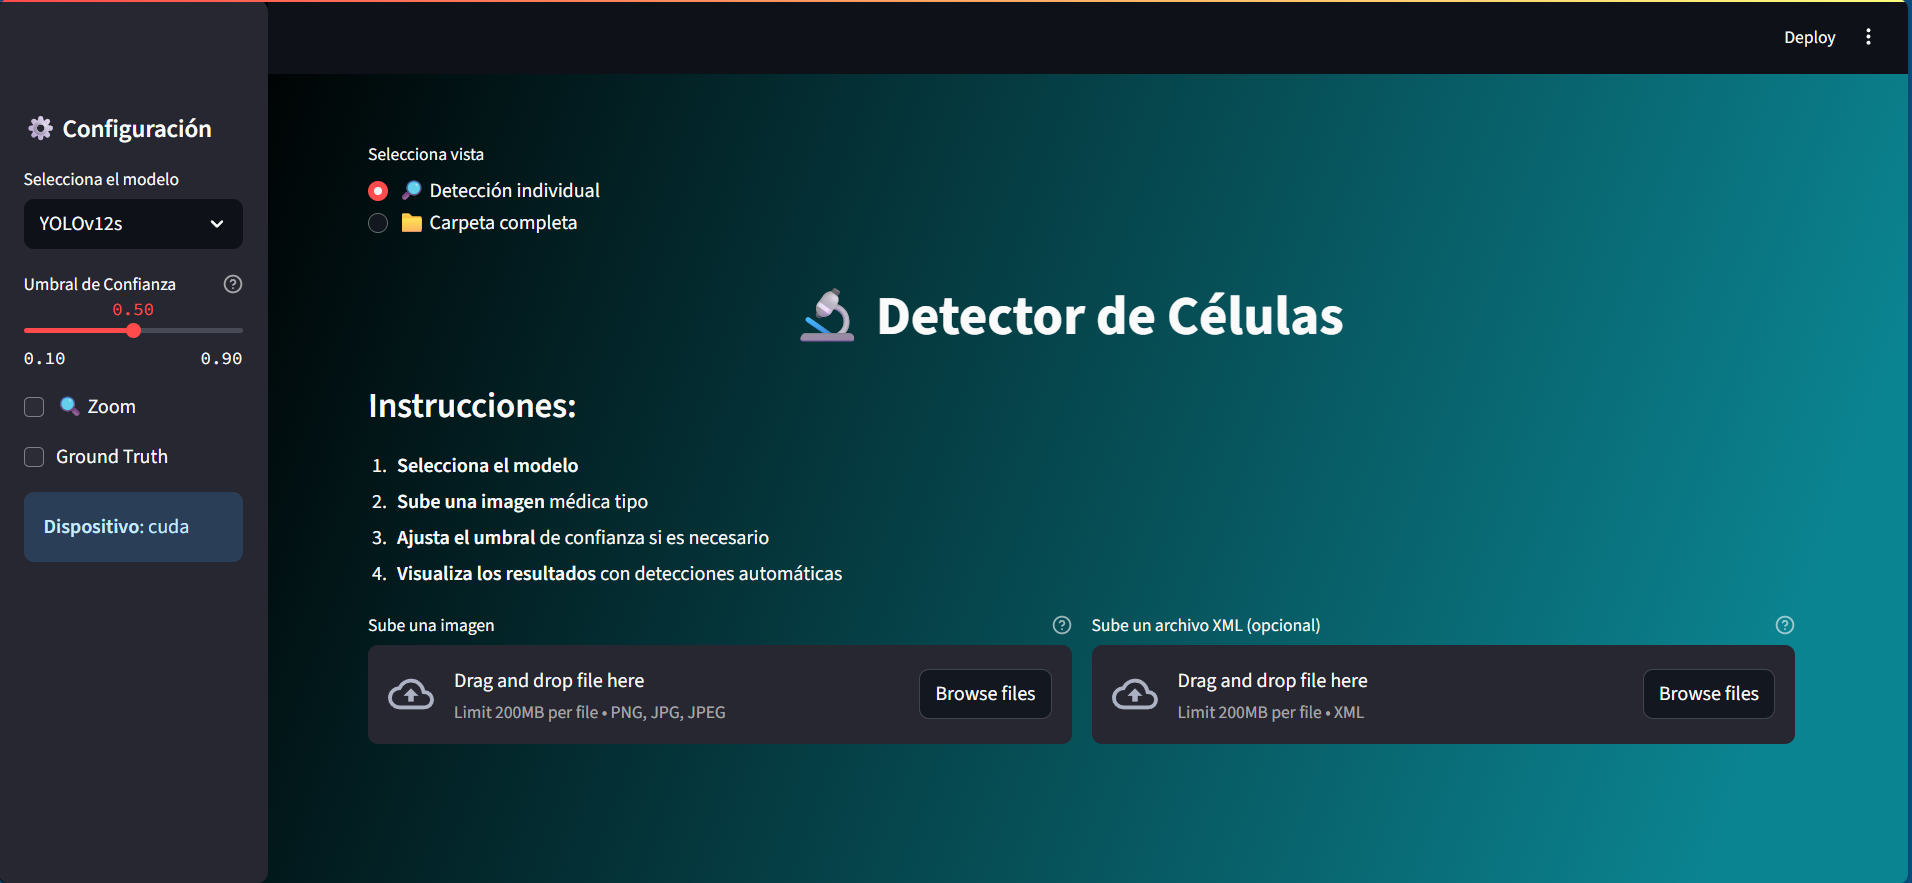
\includegraphics[width=1.0\textwidth]{figuras/app/cell_app.png}
  \caption{Interfaz de la aplicación web.}
  \label{fig:cell_app}
\end{figure}

En este punto, el usuario puede tomar la decisión de procesar una imagen individual o un conjunto de imágenes. Para esto, 
tenemos el \textit{widget} que permite la selección entre "Detección individual" o "Carpeta completa". En ambos casos,
la aplicación nos muestra una guia básica de funcionamiento como se puede apreciar en el apartado "Introducciones" de la imagen anterior.
De manera totalmente opcional, el usuario puede cargar junto a la imagen a estudio, el correspondiente conjunto de anotaciones.

El \textit{widget} de Configuración permite la seleccion manual del modelo a través de un desplazable, el umbral de confianza de IoU, 
la representación \textit{ground truth} (siempre que exista el xml asociado a la imagen) mediante un \textit{checkbox} (Figura \ref{fig:cell_app_gt}) y realizar un análisis exploratorio
sobre la imagen con un zoom (Figura \ref{fig:cell_app_zoom}). Asimismo, muestra el dispositivo (CPU,GPU) con el que se van a procesar las imágenes.

\begin{figure}[htbp]
  \centering
  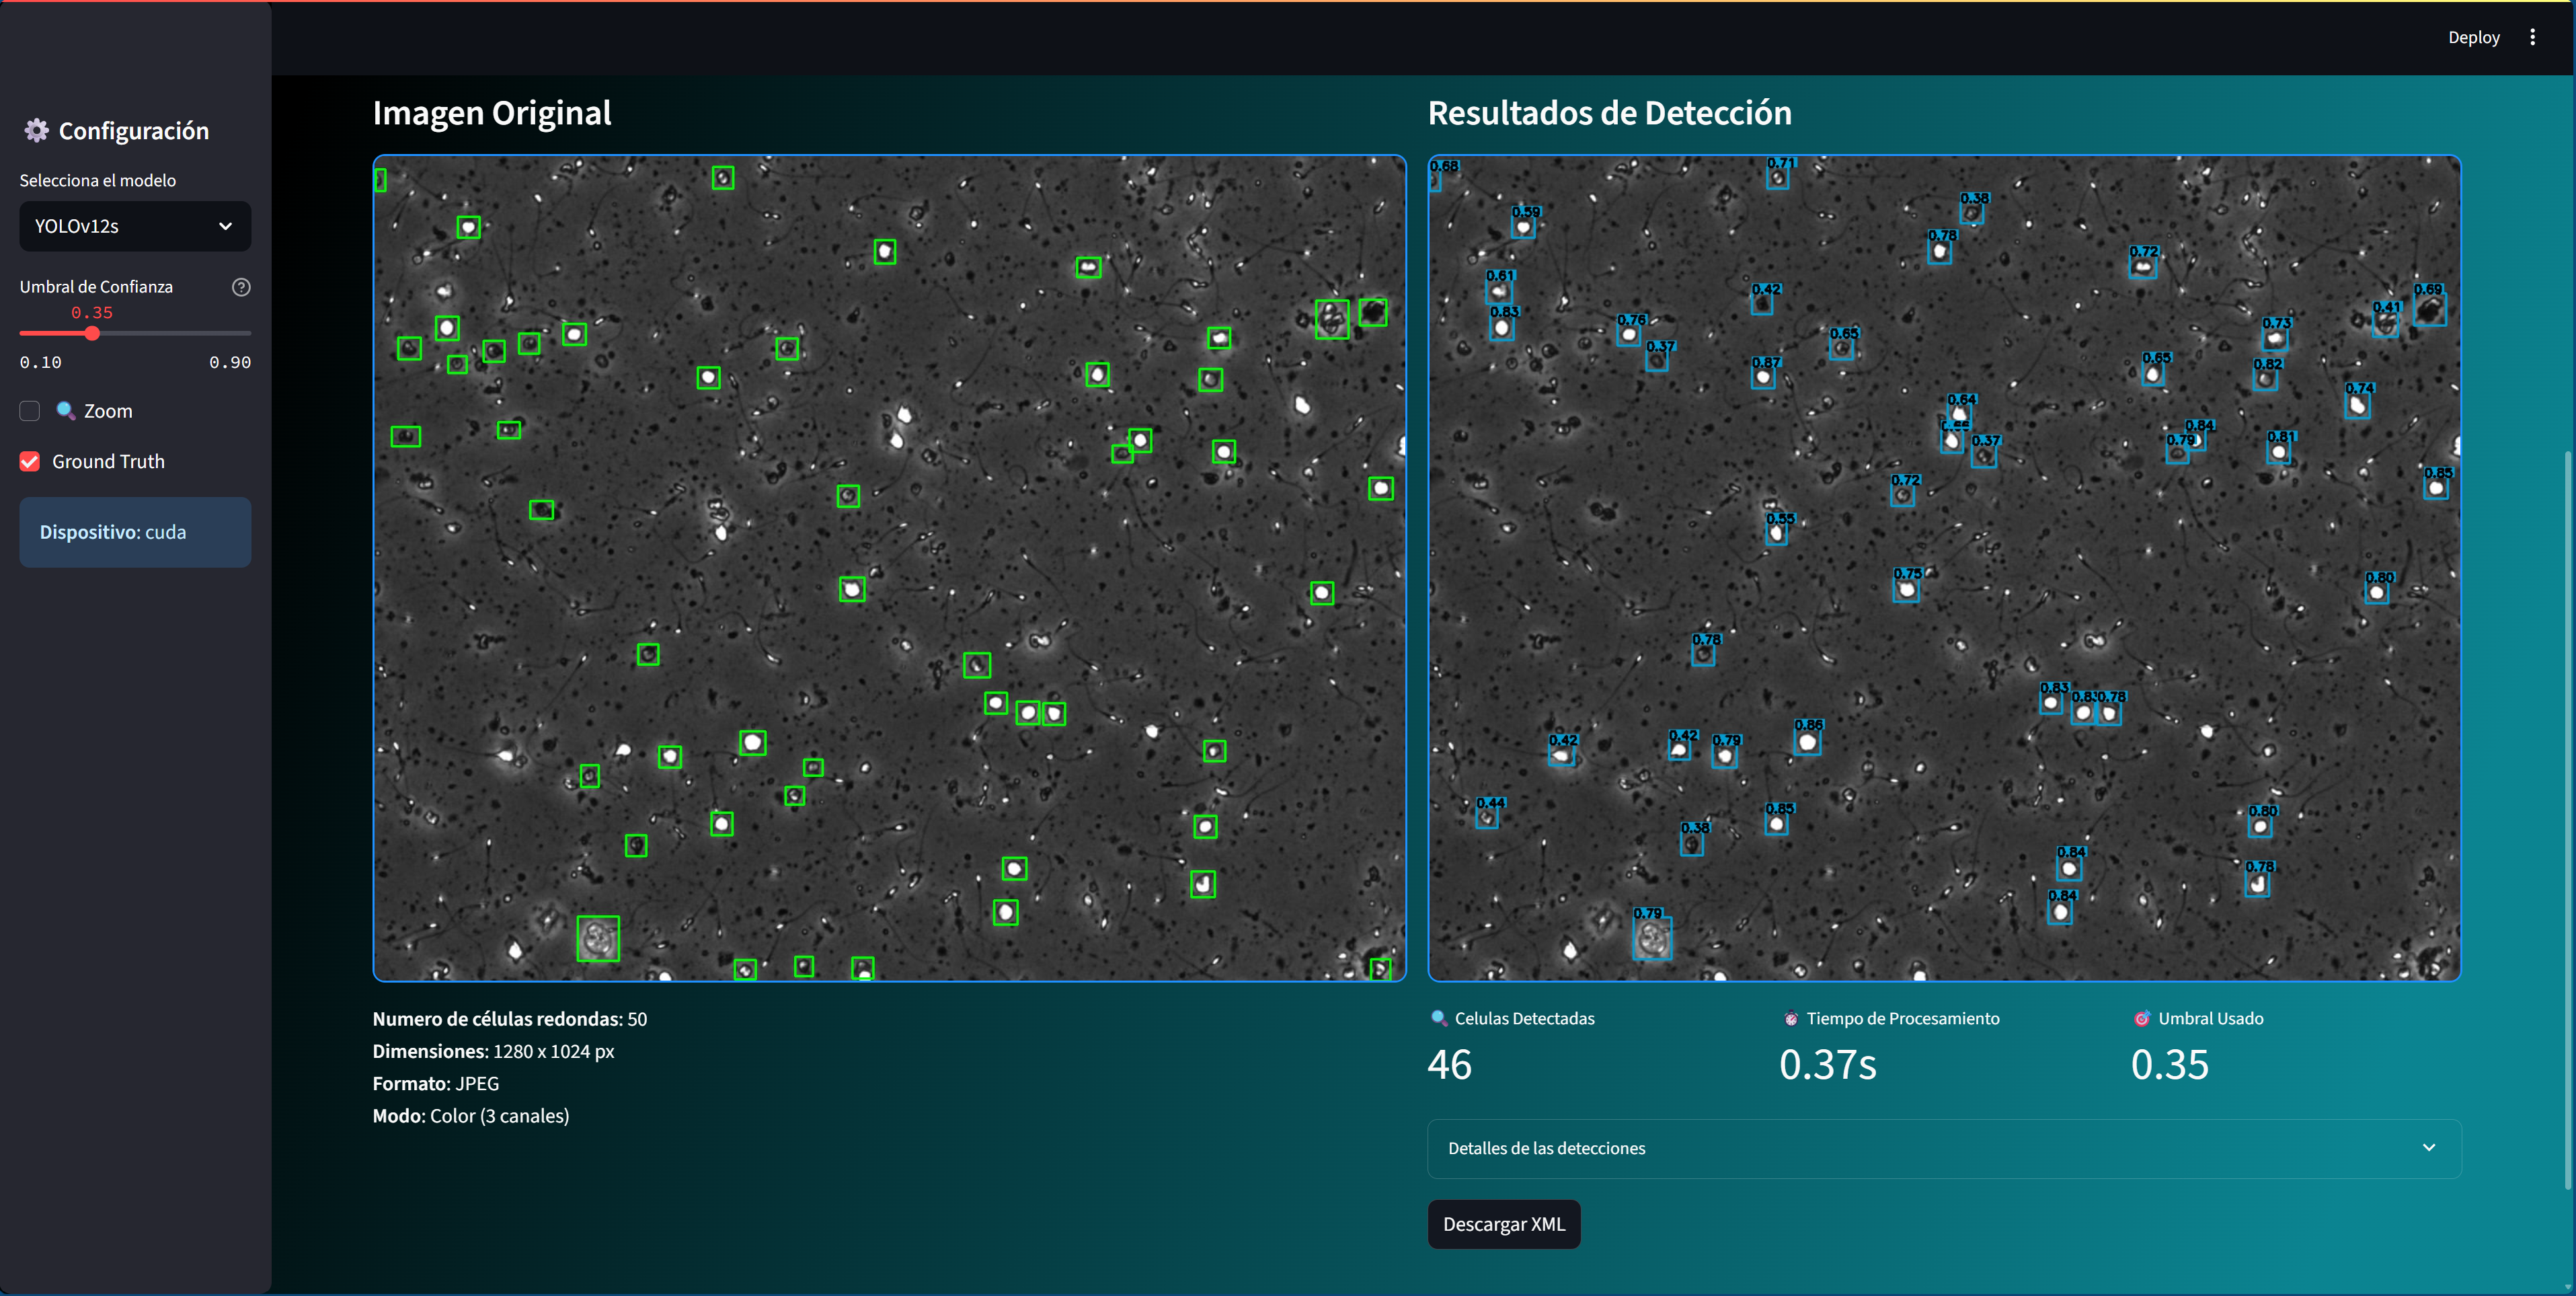
\includegraphics[width=1.0\textwidth]{figuras/app/prueba_imagen.png}
  \caption{Herramienta web: \textit{checkbox ground truth}.}
  \label{fig:cell_app_gt}
\end{figure}

\begin{figure}[htbp]
  \centering
  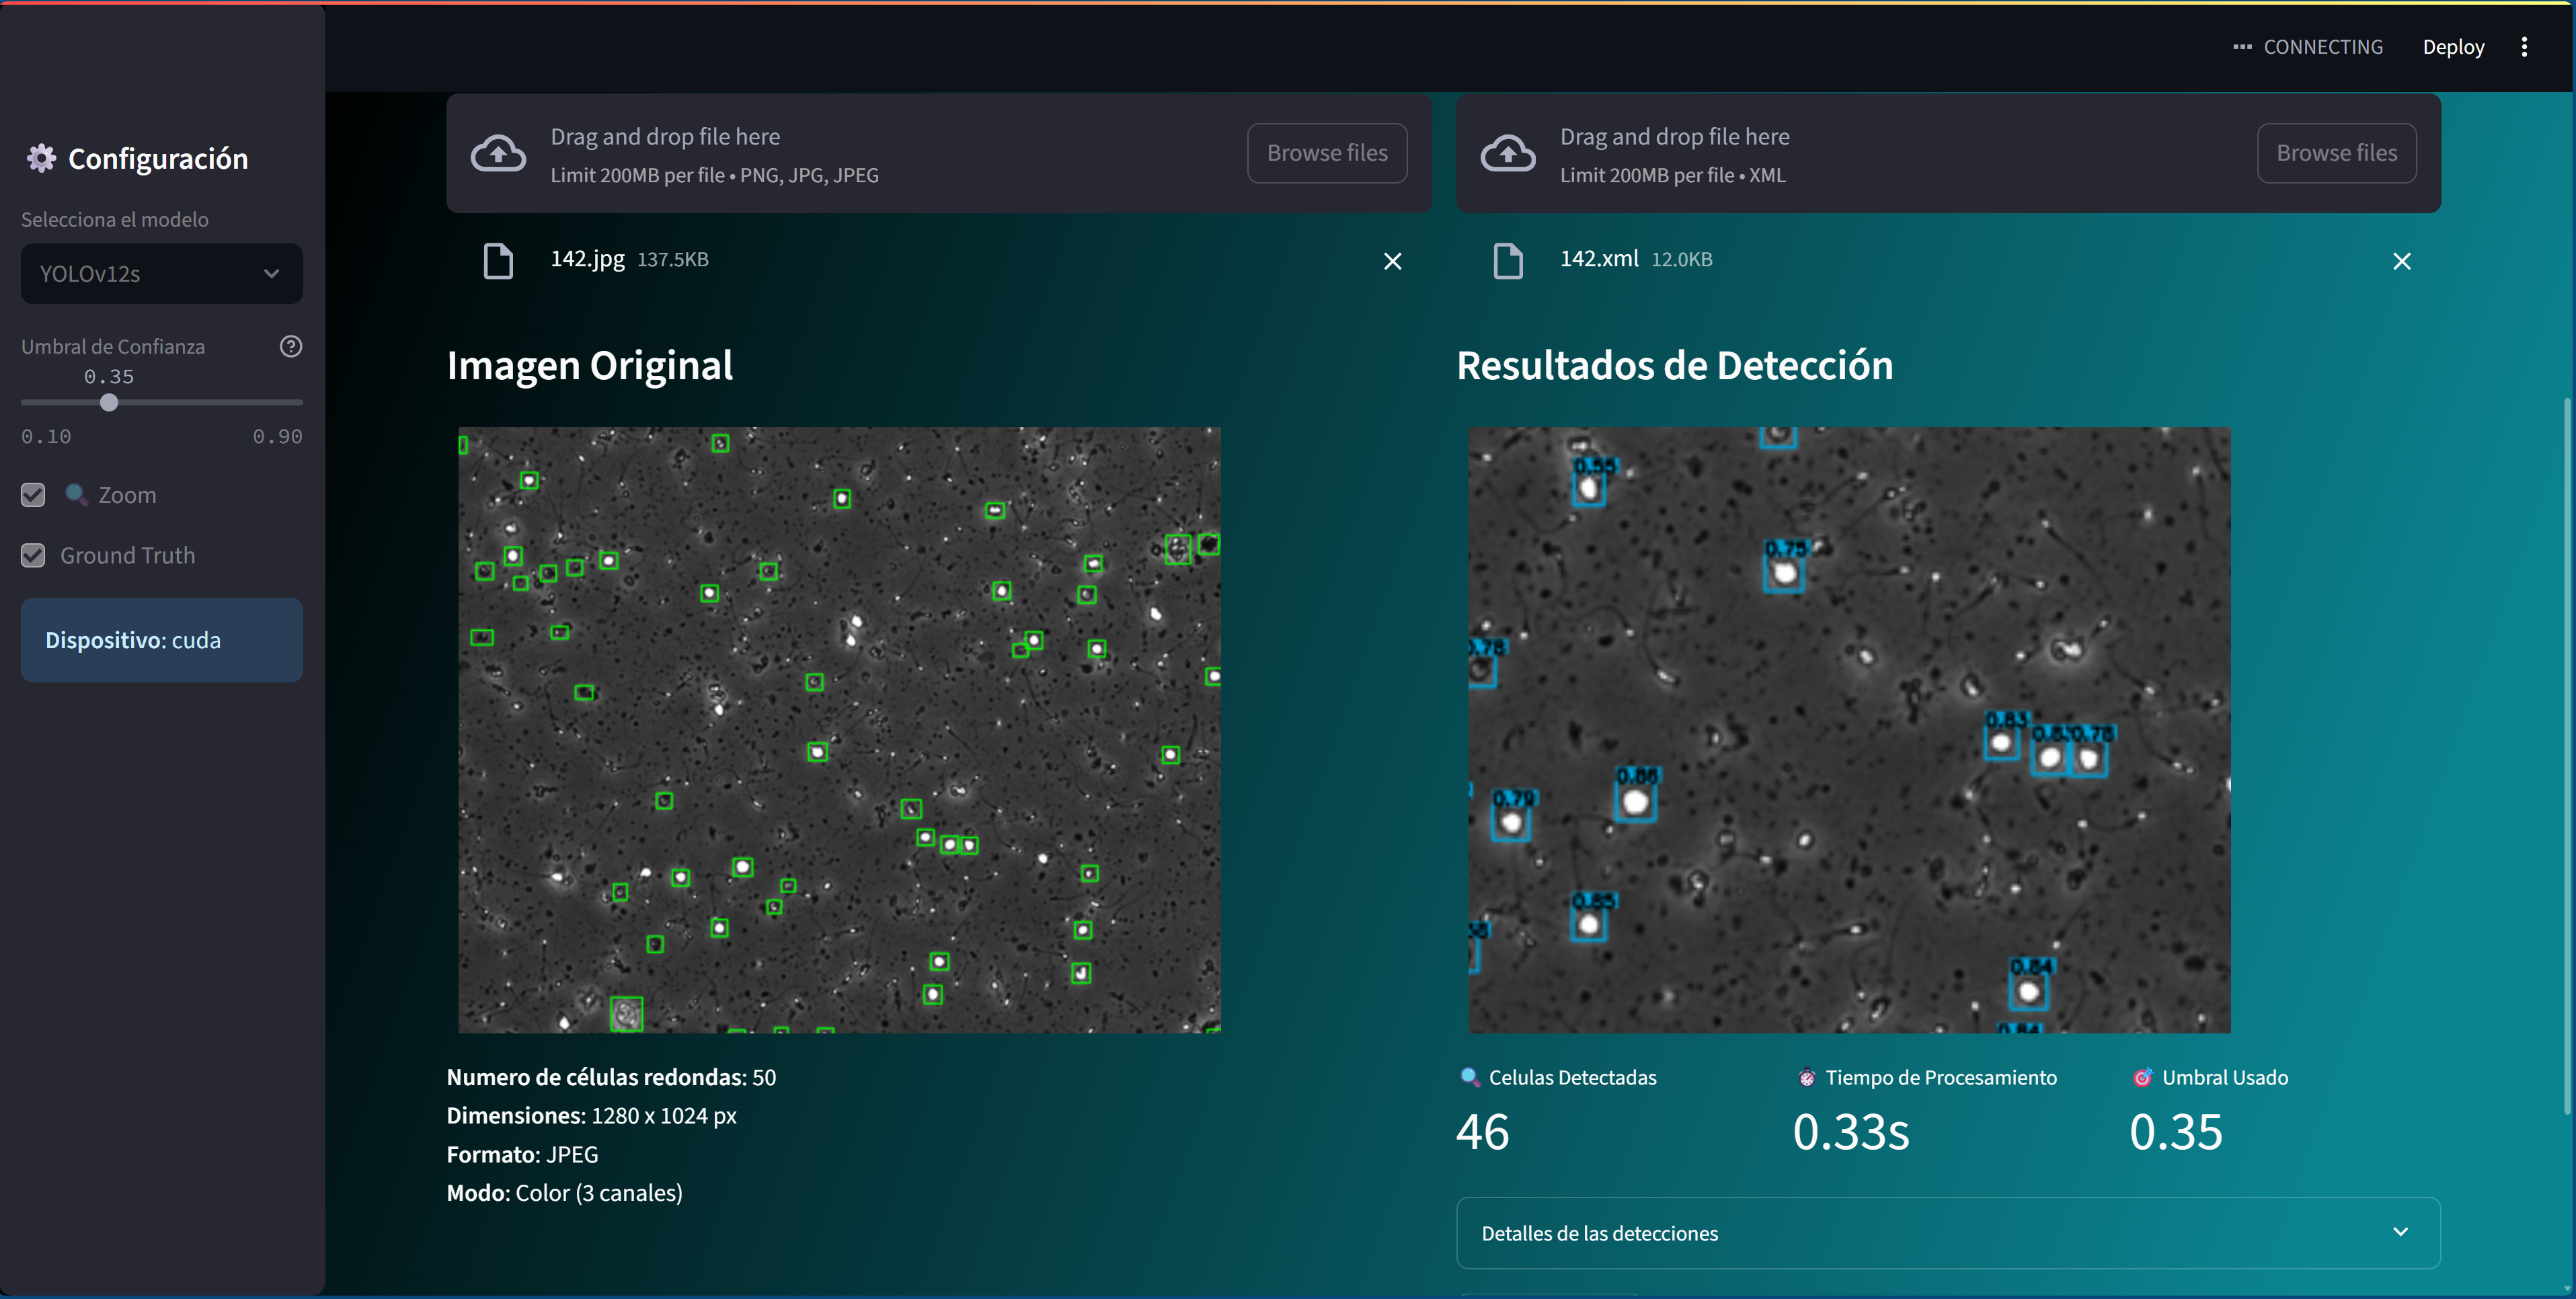
\includegraphics[width=1.0\textwidth]{figuras/app/zoom_imagen.png}
  \caption{Herramienta web: \textit{checkbox zoom}.}
  \label{fig:cell_app_zoom}
\end{figure}

Cabe destacar el \textit{widget} "Descargar XML" que permite al usuario descargar las prediciones del modelo realizadas sobre la imagen de entrada en un formato
PascalVOC. Además, 

Por el contrario, si el usuario prefiere evaluar un conjunto de imágenes con sus respectivas anotaciones, se debe seleccionar la elección de "carpeta completa" como se muestra en la Figura \ref{fig:cell_app_directory}.

\begin{figure}[htbp]
  \centering
  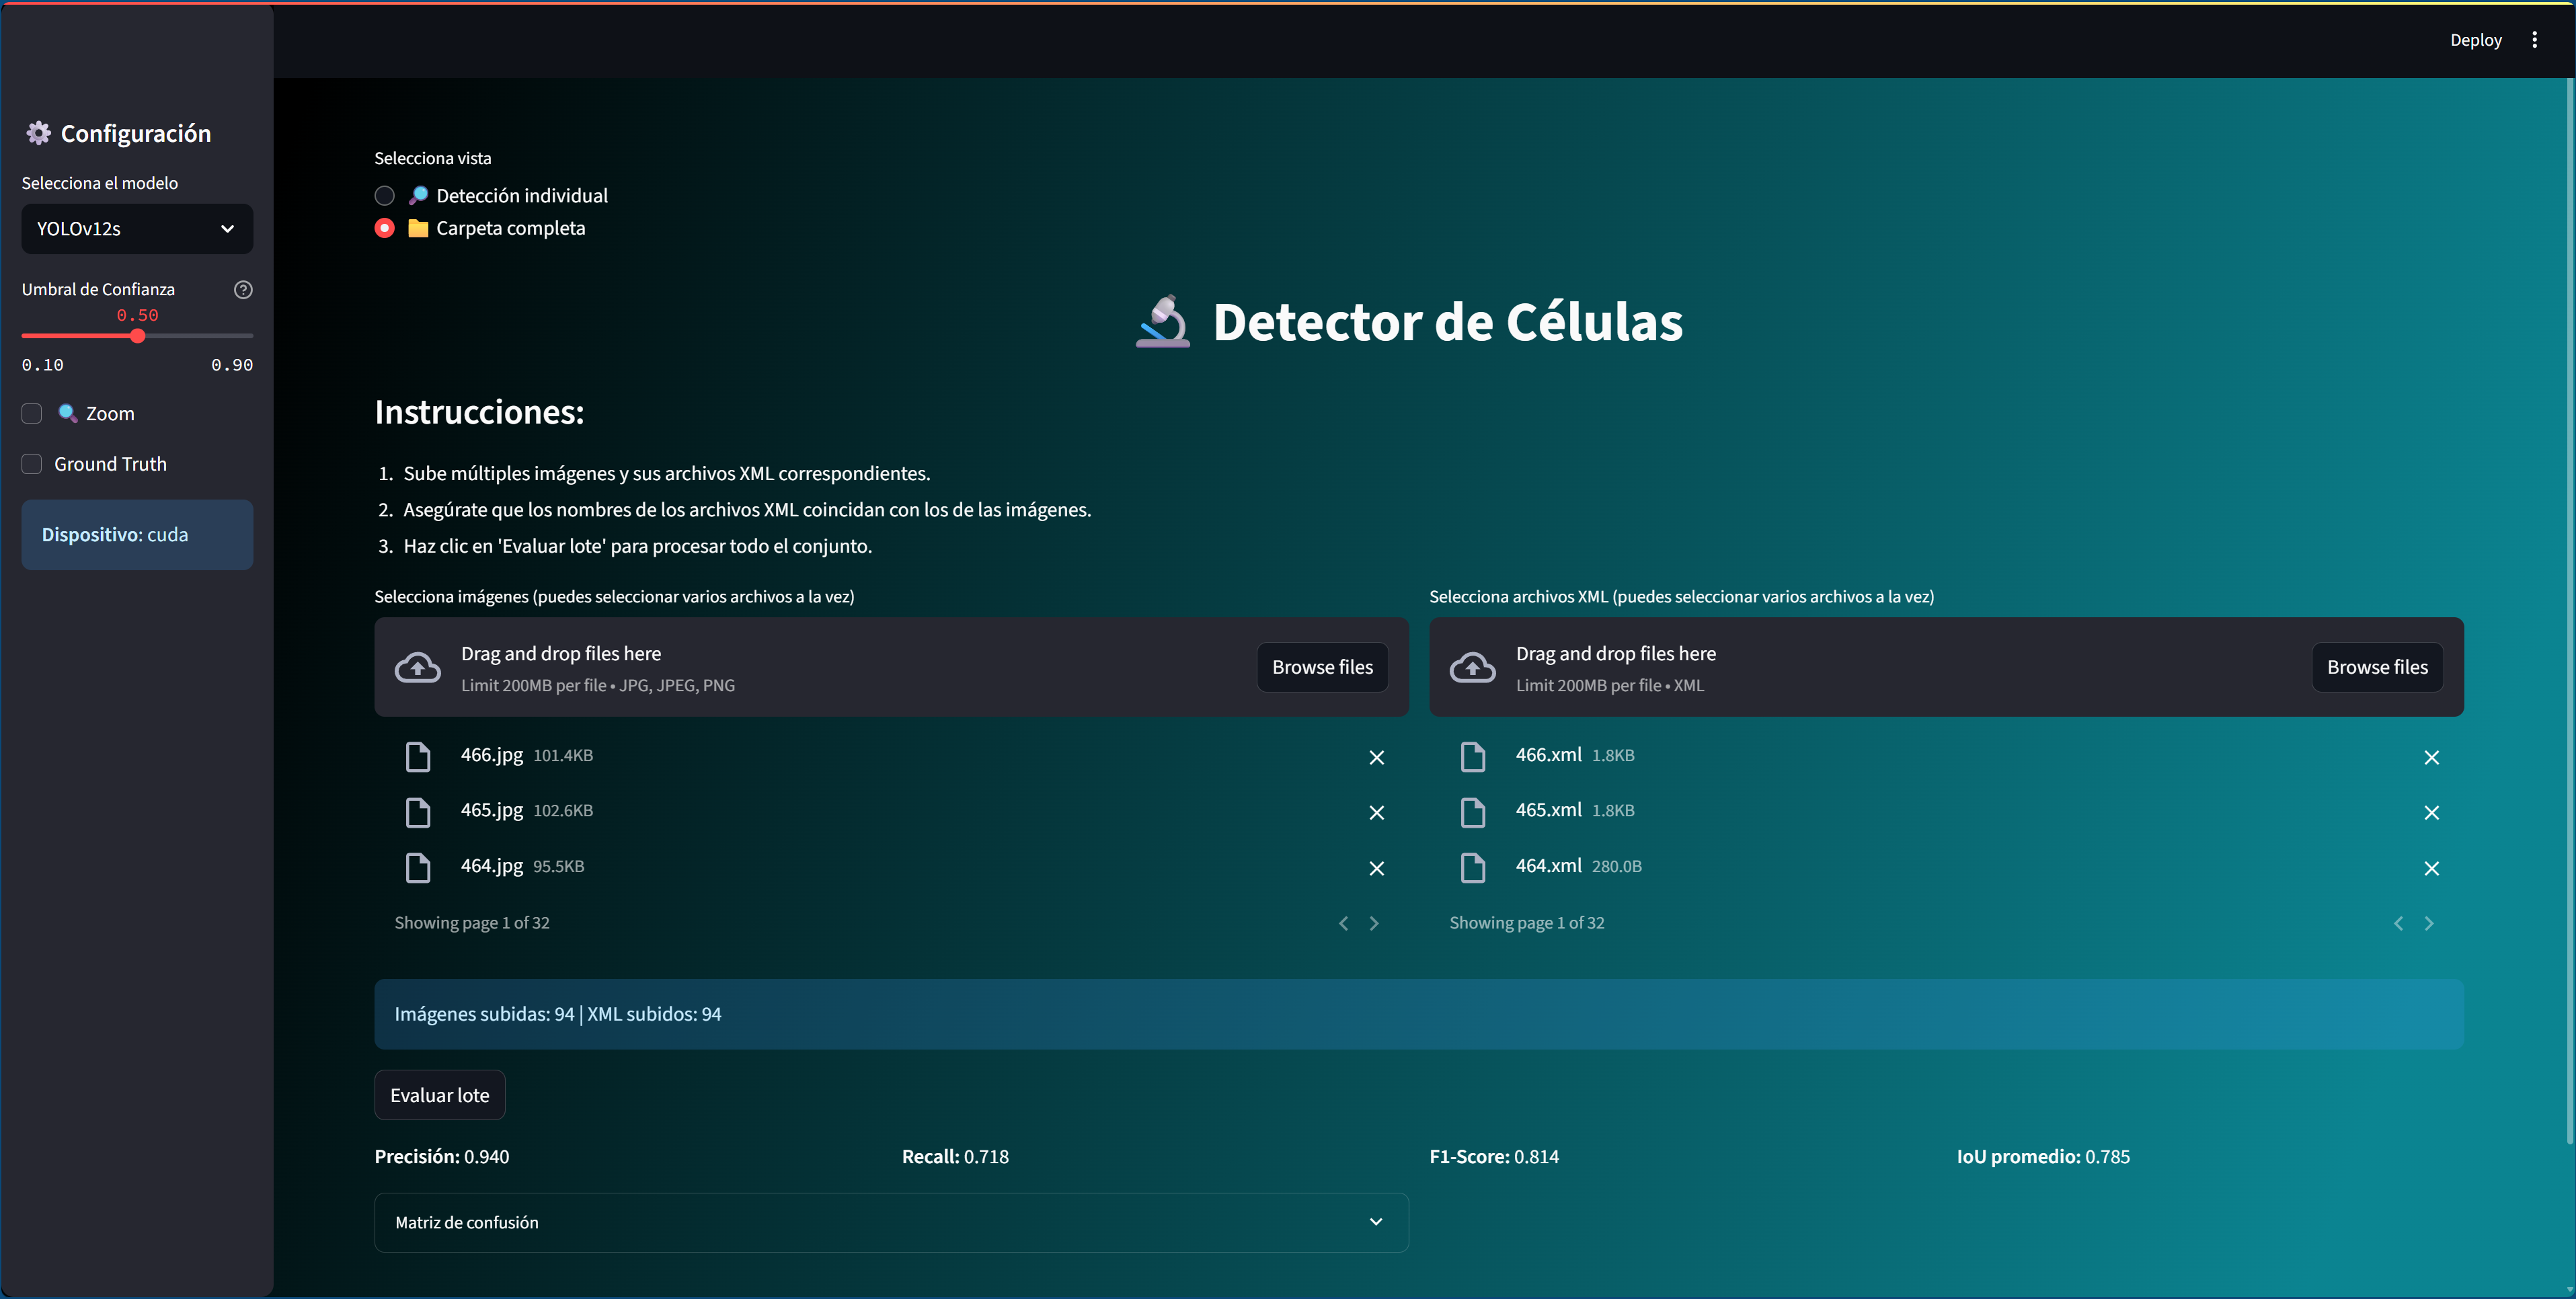
\includegraphics[width=1.0\textwidth]{figuras/app/cell_app_directorio.png}
  \caption{Herramienta web para procesar un conjunto de imágenes.}
  \label{fig:cell_app_directory}
\end{figure}

Este es un modo de evaluación, no está permitido el uso de los \textit{widgets}: \textit{ground truth} y \textit{zoom}. Sín embargo, 
el procesamiento del modelo seleccionado junto con su correspondiente umbral de procesamiento de IoU, está acompañado de un pequeño conjunto de métricas:
\textit{precision}, \textit{recall} y \textit{mAP}. Para una mejor evaluación, la herramienta muestra una matriz de confusión (Figura \ref{fig:cell_app_metrics}).

\begin{figure}[htbp]
  \centering
  \includegraphics[width=1.0\textwidth]{figuras/app/matriz_confusión.png}
  \caption{Herramienta web: métricas y matriz de confusión.}
  \label{fig:cell_app_metrics}
\end{figure}

\section{Recomendaciones de uso}
\label{sec:Recomendaciones de uso}
A continuación, se recogen pautas prácticas para el uso correcto funcionamiento de la herramienta web.

\begin{itemize}
  \item \textbf{Entorno recomendado:} se recomienda usar un entorno conda para tener aisladas las dependencias del proyecto y evitar así conflictos entre dependencias. 
  Desde el directorio \texttt{04.Code} se proponen dos alternativas:
    \begin{itemize}
      \item Instalación del entorno completo con conda (Recomendado):
        \begin{itemize}
          \item \texttt{conda env create -f environment.yml}
          \item \texttt{conda activate tfm\_env}
        \end{itemize}
      \item Instalación de un subconjunto de dependencias con conda:
        \begin{itemize}
          \item \texttt{conda create -n tfm\_env python=3.11 -y}
          \item \texttt{conda activate tfm\_env}
          \item \texttt{pip install -r 04.Codigo/requirements.txt}
        \end{itemize}
    \end{itemize}
  \item \textbf{Ejecución de la aplicación:} en la carpeta \texttt{04.Codigo/cell\_detection\_App} ejecutar:
    \begin{itemize}
      \item \texttt{streamlit run app.py}
      \item Automáticamente se abre en el navegador por defecto la URL que Streamlit indique (por defecto \texttt{http://localhost:8501}).
    \end{itemize}
  \item \textbf{Compatibilidad con modelos:} funciona únicamente con modelos de YOLO. 
\end{itemize}

\section{Resolución de problemas}
\label{sec:Resolución de problemas}
Posibles problemas que pueden tener lugar durante la instalación:

\begin{itemize}
  \item \textbf{La app no arranca / Streamlit muestra error:}
    \begin{itemize}
      \item Verificar dependencias: \texttt{pip install -r 04.Codigo/requirements.txt}
      \item Comprobar la salida en el terminal donde se ejecuta \texttt{streamlit run app.py} y revisar trazas de error.
      \item Borrar caché de Streamlit: \texttt{streamlit cache clear}.
    \end{itemize}
  \item \textbf{Modelo no encontrado o error de carga de pesos:}
    \begin{itemize}
      \item Confirmar que el fichero de pesos existe en \texttt{models/} y que la ruta es correcta (\path{04.Codigo/cell_detection_App/models/}).
    \end{itemize}
  \item \textbf{Problemas con GPU / CUDA:}
    \begin{itemize}
      \item Comprobar estado de la GPU: ejecutar \texttt{nvidia-smi} en terminal.
      \item Verificar que PyTorch detecta la GPU: 
        \begin{itemize}
          \item \texttt{python -c "import torch; print(torch.cuda.is\_available())"}
        \end{itemize}
      \item Si falla, forzar ejecución en CPU desde la UI o variable de entorno: \texttt{CUDA\_VISIBLE\_DEVICES=""}.
    \end{itemize}
  \item \textbf{Errores al procesar imágenes / XML mal formados:}
    \begin{itemize}
      \item Validar que las imágenes están en formatos soportados (\texttt{.jpg, .jpeg, .png}) y que los XML cumplen con el formato PascalVOC.
      \item Revisar el log de parsing en \texttt{04.Codigo/cell\_detection\_App/utils/} y corregir los ficheros señalados.
    \end{itemize}
\end{itemize}

\end{document}


% ¿Eliminar el bloque de validación de configuración y dejarlo solo pra el optuna, entrenamiento, validación cruzada, data augmentaion?
% En Resultados, quitar Fast-RCNN y a parte añadir aquí los resultados para yolo y custom de validacion cruzada.
% Si finalmente voy mejor, añado lo de Fast-RCNN
% ¿Que comento en metodología, un poco el procedimiento de cada pipeline?